% add option draft to skip images
\documentclass[12pt,a4paper,twosided,openany]{scrbook}
%\documentclass[12pt,a4paper,twosided,open=right]{scrbook}
% \documentclass[12pt,a4paper,twosided,open=right,draft]{scrbook}

% Entwickelt auf Basis von Carsten Kerns Template.

\usepackage[backend=biber,style=alphabetic,maxalphanames=60,maxbibnames=10]{biblatex}
% \usepackage[backend=bibtex,style=alphabetic]{biblatex}
% \usepackage{natbib}
\usepackage[ngerman]{babel}
\usepackage[utf8]{inputenc}
\usepackage{csquotes}
\usepackage{ifthen}
\usepackage{xargs}
\usepackage{amsmath}
\usepackage{amsfonts}
\usepackage{amssymb}
\usepackage{graphicx}
\usepackage{svg}
% \usepackage{fancyhdr}
\usepackage{tabularx}
\usepackage{geometry}
\usepackage{setspace}
\usepackage[right]{eurosym}
\usepackage[printonlyused]{acronym}
\usepackage{subfig}
\usepackage{floatflt}
%\usepackage{color}
\usepackage{xcolor}
\usepackage{colortbl}
\usepackage{paralist}
\usepackage{array}
\usepackage{multirow}
% \usepackage{titlesec}
\usepackage{parskip}
% \usepackage[subfigure,titles]{tocloft}
\usepackage[pdfpagelabels=true,colorlinks=true,linkcolor=black,anchorcolor=black,citecolor=black,filecolor=black,menucolor=black,runcolor=black,urlcolor=black]{hyperref}
\usepackage{booktabs}
\usepackage[lighttt]{lmodern}
\usepackage{mathabx}

\usepackage{listings}
\lstset{basicstyle=\footnotesize, captionpos=b, breaklines=true, showstringspaces=false, tabsize=2, frame=lines, numbers=left, numberstyle=\tiny, xleftmargin=2em, framexleftmargin=2em}

\geometry{a4paper, top=27mm, left=25mm, right=15mm, bottom=27mm, headsep=10mm, footskip=12mm}

% make lstinline be normalsize but keep displayed listings small
\makeatletter
\lstdefinestyle{mystyle}{
  basicstyle=%
    \ttfamily
    \lst@ifdisplaystyle\scriptsize\fi
}
\makeatother

\lstset{
	language=C++,
	% basicstyle=\ttfamily\scriptsize,
	style = mystyle,
	% basicstyle=\ttfamily\scriptsize,
	keywordstyle=\bfseries\ttfamily,
	% commentstyle=\color{LimeGreen}\ttfamily,
	commentstyle=\color{gray}\ttfamily,
	emphstyle={\color{Purple!90!black}},
	tabsize=4,
	morekeywords={nullptr,nullptr_t,vector,string,std,list,map,pair,set,size_t,endl,cout,move},
	emph={},
	showstringspaces=false,
}

\setcapindent{0pt}
\setkomafont{captionlabel}{\bfseries}

\DefineBibliographyStrings{ngerman}{
	andothers = {{et\,al\adddot}},
}


\DeclareLabelalphaTemplate{
  \labelelement{
    \field[final]{shorthand}
    \field{label}
    \field[strwidth=3,strside=left,ifnames=1,names=1]{labelname}
    \field[strwidth=1,strside=left,names=1-3]{labelname}
  }
  \labelelement{
    \field[strwidth=2,strside=right]{year}
  }
}
\renewcommand*\labelalphaothers{$^\Asterisk\mkern-.8mu$}

\newcommandx{\student}[3][]{
	\def\studentName{#1}%
	\def\studentMatnr{#2}%
	\def\studentStudiengang{#3}%
}

\newcommandx{\MyTitelseite}[8][]{
\thispagestyle{empty}
\ifthenelse{\equal{#1}{}}{
	
\includegraphics[scale=0.2]{lib/oth-logo.png}
}{
	
\includegraphics[scale=0.2]{lib/oth-logo.png}\hfill\includegraphics[scale=0.5]{#1}
}
\begin{center}
\ifthenelse{\equal{#2}{2}}{ % then
	\vspace*{2cm}
	\Large
	\textbf{Ostbayerische Technische Hochschule Regensburg}\\
	\textbf{Fakultät für Informatik und Mathematik}\\
	\vspace*{2cm}
	\Huge
	\textbf{#3}\\[1em]
	\large
	Zur Erlangung des akademischen Grades des\\
	\ifthenelse{\equal{#3}{Bachelorarbeit}}{Bachelor of Science (B.Sc.)}{Master of Science (M.Sc.)}\\
	\vspace*{1cm}
	\Large
	\textbf{#4}\\
}{ % else
	\vspace*{1cm}
	\Large
	\textbf{#4}\\
	\vspace*{2cm}
	\large
	An der Fakultät für Informatik und Mathematik der\\
	Ostbayerischen Technischen Hochschule Regensburg\\
	im Studiengang\\[2em]
	\textbf{\studentStudiengang}\\[2em]
	eingereichte\\
	\vspace*{1cm}
	\Large
	\textbf{#3}\\[2em]
	\large
	zur Erlangung des akademischen Grades des\\
	\ifthenelse{\equal{#3}{Bachelorarbeit}}{Bachelor of Science (B.Sc.)}{Master of Science (M.Sc.)}
	\vspace*{1cm}
	\Large
}
	\vfill
	\normalsize
	%\newcolumntype{x}[1]{>{\raggedleft\arraybackslash\hspace{0pt}}p{#1}}
	\begin{tabular}{rl}%{6cm}p{7.5cm}}
	    \rule{0mm}{1ex}\textbf{Vorgelegt von:} & \studentName \\
		\rule{0mm}{1ex}\textbf{Matrikelnummer:} & \hspace*{-0.5em}\begin{tabular}[t]{r}\studentMatnr\end{tabular} \\ 
		\ifthenelse{\equal{#2}{1}}{~\\}{\rule{0mm}{1ex}\textbf{Studiengang:} & \studentStudiengang \\[2em]}
		\rule{0mm}{1ex}\textbf{Erstgutachter:} & #5 \\ 
		\rule{0mm}{1ex}\textbf{Zweitgutachter:} & #6 \\[2em]
		\rule{0mm}{1ex}\textbf{Abgabedatum:} & #7 \\ 
	\end{tabular} 
\end{center}
\pagebreak
}



% ein paar nützliche Kommandos

\newcommand\defsec[1]{\label{sec:#1}}
\newcommand\refsec[1]{\ref{sec:#1}}

%\newcommand\todo[1]{\textcolor{red}{[{\textbf{TODO}} #1]}}
\newcommand\todo[1]{} % remove todos

%\newcommand\new[1]{\textcolor{new}{{#1}}}
\newcommand\new[1]{#1} % plain text
%\newcommand\old[1]{\textcolor{gray}{{\sout{#1}}}}
\newcommand\old[1]{} % remove old stuff

\definecolor{lgdv}{rgb}{.80,.23,.13}
\definecolor{agreen}{rgb}{.2,.8,.2}
\definecolor{jorange}{rgb}{.9,.6,.0}
\definecolor{new}{rgb}{.8,.4,.4}

\newcommand\NOTE[3]{\textcolor{#1}{[#2: #3]}}
\newcommand{\TODO}[1]{\\ \colorbox{yellow}{TODO: #1}\\}

%\newcommand\kai[1]{\NOTE{lgdv}{Kai}{#1}}
\newcommand\kai[1]{} % remove notes
%\newcommand\niko[1]{\NOTE{jorange}{Niko}{#1}}
\newcommand\niko[1]{} % remove notes

\newcommand\To{\ensuremath{\to}}
\newcommand\hi[1]{\textcolor{red}{#1}}

\let\shortcite=\cite

\addbibresource{bib.bib}

\begin{document}

% ----------------------------------------------------------------------------------------------------------
% Titelseite
% ----------------------------------------------------------------------------------------------------------
\newcommand{\stud}{Emanuel Erben}  % Ihr Name
\student{\stud}
{3174817}						% Matrikelnummer
{Informatik}					% Studiengang

\MyTitelseite{}					% Optionales Logo des extern betreuenden Unternehmens
% \MyTitelseite{pics/mathcomm}	% Optionales Logo des extern betreuenden Unternehmens
{1}								% Style der Titelseite (1 oder 2)
{Bachelorarbeit}				% Typ der Abschlussarbeit (\in {Bachelorarbeit, Masterarbeit})
{Vergleich verschiedener Ansätze der Multiplattform Applikationsentwicklung anhand einer Beispiel-Anwendung}				% Thema der Arbeit						
{Prof.\ Dr.-Ing.\ Kai Selgrad}		% Betreuer
{Prof.\ Dr.\ Name des Zweitgutachters}	% Zweitgutachter
{15.09.\the\year}				% Abgabedatum

\thispagestyle{empty}
~\pagebreak

\setcounter{page}{1} 

Das muss an den Kapiteln noch gemacht werden:

0.Abstract:
Ende nochmal umschreiben
1.Motivation:
Einordnung nochmal anschauen und insgesamt überarbeiten.
Die Arbeitsbeschreibung

Related:
Überarbeiten und eventuell Performance Untersuchung mit neuem Austauschen.

3.Grundlagen:
Projektbeschreibung : 
noch machen
Themenabgrenzung :
Mal schauen ob noch mehr und bei Spiel Ende nochmal nachschauen.
Erklärung warum nur Smartphone Applikationen betrachtet.
Begriffe:
umstellen
Arten:
Nativ und Hybrid soweit an Selgrad, Rest muss überareiten
drüberlesen

4. Einleitung
Vielleicht nochmal bisl spannender
4.1 Nativ

4.2 hybrid

4.3 Flutter
ausmisten
ordentlich neu schreiben

4.4 hybrid flutter

5.Auswertung
Noch komplett
kriterien aussuchen
Werte zusammenschreiben, messen oder nachforschen
Tabellen und sonstiges erstellen

6.Fazit
Noch komplett


% ----------------------------------------------------------------------------------------------------------
% Abstract
% ----------------------------------------------------------------------------------------------------------
% \thispagestyle{empty}
\setstretch{1.15} % Zeilenspacing
\chapter*{Abstract}

\bigskip 

In den letzten Jahren nutzen viele Leute nicht mehr ihren Computer sondern vor allem ihre Smartphones und andere mobile Endgeräte, um auf verschiedenen Dienste, Konten und Online-Anwendungen zuzugreifen. Um eine Anwendung auf verschiedenen Plattformen veröffentlichen zu können haben Entwickler unterschiedliche Möglichkeiten. Diese reichen dabei von der Entwicklung einer eigenen Anwendung für jede einzelne Plattform bis hin zu einem Code der für die verschiedenen Plattformen genutzt werden kann. Dadurch ist die Wahl des richtigen Entwicklungsansatzes und der Technologie schwer, da jeder Ansatz seine Vor- und Nachteile hat. 

In dieser Arbeit werden vier verschiedene Applikationen, die mit unterschiedlichen Ansätzen implementiert wurden, beschrieben und analysiert. Danach werden die Ergebnisse der verschiedenen Untersuchungen vorgestellt und verglichen. Dabei wird darauf eingegangen, welche Vor- und Nachteile die einzelnen Implementierungen für die betrachteten Kriterien haben. Der Schwerpunkt der Arbeit liegt dabei auf der Android Plattform und speziell den Programmiersprachen Kotlin und Dart. Die vier Implementierungen sind eine native, hybride, cross-kompilierte und eine cross-kompilierte Applikation mit Webanteil, also einem Mix aus hybridem und cross-kompilierten Ansatz.

\frontmatter

% ----------------------------------------------------------------------------------------------------------
% Inhaltsverzeichnis
% ----------------------------------------------------------------------------------------------------------
\tableofcontents
\vfill
\pagebreak

% % ----------------------------------------------------------------------------------------------------------
% % Abbildungsverzeichnis
% % ----------------------------------------------------------------------------------------------------------
\listoffigures
\vfill
\pagebreak
% 
% % ----------------------------------------------------------------------------------------------------------
% % Tabellenverzeichnis (optional)
% % ----------------------------------------------------------------------------------------------------------
% \listoftables
% \vfill
% \pagebreak

% ----------------------------------------------------------------------------------------------------------
% Listingsverzeichnis (optional; Code nur, wenn wirklich sinnvoll und wichtig)
% ----------------------------------------------------------------------------------------------------------
%\lstlistoflistings
%\vfill
%\pagebreak


% ----------------------------------------------------------------------------------------------------------
% Inhalt
% ----------------------------------------------------------------------------------------------------------
\setstretch{1.15}


\mainmatter

\chapter{Motivation}
Wenn eine Applikation entwickelt werden soll, ist die Wahl der richtigen Methode, Frameworks oder auch der Programmiersprache eine wichtige Entscheidung für das Projekt. Viele Entscheidungen können im Verlauf der Entwicklung noch einfach geändert werden, aber um eine derartige Entscheidung zu ändern, müssen Teile der Anwendung oder auch der komplette Quellcode neu geschrieben werden. Dazu kommen tausende Artikel, warum die eine neue Programmiersprache der neue Standard ist. So ist eine derartig wichtige Entscheidung oft sehr schwierig.

Da oft Anwendungen nicht nur auf einem Gerätetyp laufen sollen, sondern allen Nutzern auf den verschiedensten Plattformen zur Verfügung stehen soll, hat diese Entscheidung noch einmal eine größere Bedeutung, da sie auch eng verbunden mit den Kosten der Entwicklung und der Erfahrung durch den Nutzer ist.

In Zeiten der Heimcomputer und des stetig wachsenden Internets war der einfachste Weg , eine Webseite zu entwickeln, die über den Browser der genutzten Geräte aufgerufen werden konnte. Mit der Ära der Smartphones jedoch änderte sich das. So waren Webapplikationen oft nicht für die Nutzung an derartig kleinen Geräten mit einer Toucheingabe angepasst.

Die Nutzung von Smartphones öffnete außerdem die Tür, andere Funktionalitäten wie die Kamera, Bluetooth oder GPS-Daten zu nutzen. Deshalb wurden Applikationen oft mit Objectiv-C beziehungsweise Swift für iOS und Java, jedoch mittlerweile Kotlin für Android entwickelt. Mit deren Hilfe wurden native Anwendungen für das Smartphone entwickelt, die diese neuen mobilen Plattformen optimal ausnutzen konnten.

Durch den Wunsch nach einer Multi-Plattform Anwendung, also dass die App für mehrere Plattformen veröffentlicht werden soll, muss jedoch für jede Plattform eine eigene Applikationen in der jeweiligen Programmiersprache und Technologie geschrieben werden. Dadurch entsteht ein sehr hoher Aufwand und die Kosten multiplizieren sich mit der Zahl der abzudeckenden Plattform. Deswegen wurde bereits früh mit der Entwicklung von sogenannten Cross-Plattform Technologien gestartet, die es ermöglichen sollen, mit einem geteilten Code so viele Plattformen wie möglich abzudecken. So erschien 2008 etwa PhoneGap. Es war ein Open-Source Framework zur Entwicklung von hybriden mobilen Applikationen, die mit Hilfe von HTML, CSS und Javascript programmiert wurden. PhoneGap und sein Nachfolger Cordova waren einige Zeit auch sehr beliebt in diesem Bereich. 2019 hatten beide zusammen einen Marktanteil von knapp 40\% unter den Cross-Plattform Frameworks \cite{statist_CP_Framework}.

Dennoch werden viele Entwicklung immer noch nativ entwickelt. So ergab eine interne Untersuchung der Firma \verb|ScanBot SDK|\footnote{https://scanbot.io/de/blog/native-apps-vs-cross-platform/}, dass 2019 57\% ihrer Nutzer native Applikationen entwickelten, obwohl ihr Produkt ebenso für viele der gängigen Cross-Plattform Frameworks zur Verfügung steht. Außerdem kann in Blogposts von einigen größeren Unternehmen lesen, in dem sie erklären, wie sie versuchten eine  Cross-Plattform-Entwicklungen einzuführen, jedoch aus verschiedenen Gründen  wieder einstellten. So etwa auch Airbnb \cite{Airbnb_react_goals}. Sie nutzten das von Facebook mitentwickelte Framework React Native. 2019 hatte dieses Framework einen Marktanteil von 42\%. 
\break
Ihre Ziele waren einfach:
\begin{enumerate}
    \item Schnelleres entwickeln.
    \item Die gleiche Codequalität beibehalten.
    \item Nur noch eine Codebasis.
    \item Die Entwicklererfahrung verbessern.
\end{enumerate}
Jedoch traten während der Entwicklung einige technische Probleme auf, die dazu führten, dass sie ihre Ziele nicht einhalten konnten und 2018 wieder zu einem nativen Ansatz zurückkehrten.

Durch Beispiele wie dieses, waren und sind App-Entwickler oft skeptisch gegenüber derartigen Lösungen, da dies auch immer mit großen Änderungen und hohen Investitionen verbunden sind. Dennoch ist der Wille da und auch die Zahl der Cross-Plattform Entwicklungen nimmt in den letzten Jahren zu. So ergab die Untersuchung von \verb|ScanBot SDK|, dass 2021 58\% Cross-Plattform Lösungen nutzten. Auch eine Untersuchung von Jetbrains ergab, dass 2021 53\% aller App Entwickler derartige Technologien nutzen \cite{JetBrains_miscellaneous_2021}.

\begin{figure}[ht]
  \centering
  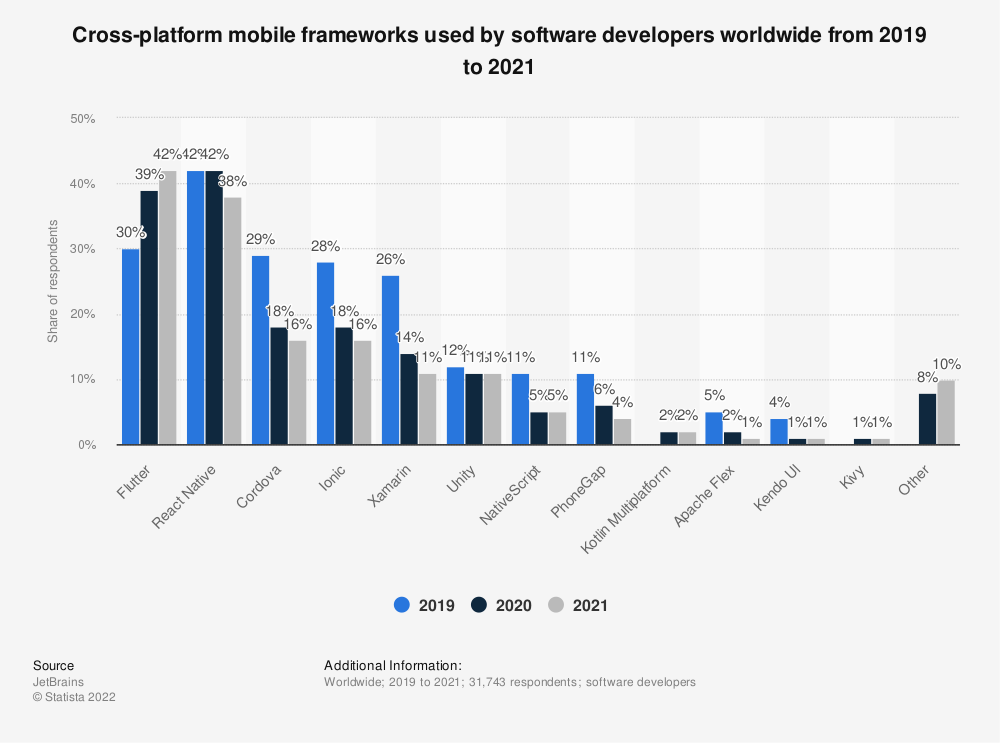
\includegraphics[height=7cm,keepaspectratio]{images/cross-platform-mobile-frameworks.png} 
  \caption[Statistik Cross-Plattform-Frameworks]{Cross-Plattform-Frameworks 2019-2021 \cite{statist_CP_Framework}}
  \label{fig:statista_cross_plattform}
\end{figure}

Diese Zahl könnte sich auch noch stark ändern. Abbildung \ref{fig:statista_cross_plattform} zeigt eine Statistik, die die Verteilung von verschiedenen Cross-Plattform-Entwicklungen zeigt. Sie zeigt eindrucksvoll wie schnell sich die Verteilung von Cross-Platform Frameworks ändern kann. Ein Framework, das hier jedoch besonders auffällt ist Flutter. Es ist ein Framework das erst 2017 auf den Markt gekommen ist und innerhalb von gerade einmal 4 Jahren auf einen Marktanteil von 42\% gekommen ist. Von einigen wird es als der neue Standard angesehen und viele Unternehmen steigen auf Flutter um oder bekunden großes Interesse daran. 

Jedoch gibt es auch Entwickler, die wegen Unsicherheiten und einigen anderen Gründen immer noch nativ entwickeln. So entwickelt die Number42 alle ihrer betreuten mobilen Applikationen mit den nativen Programmiersprachen. Auch die nativen Programmiersprachen entwickeln sich dabei stetig weiter und bekommen Änderungen, die eine Entwicklung vereinfachen und beschleunigen. Dadurch ist auch dieser Ansatz nicht von der Hand zu weisen und es kann durchaus sinnvoll sein, neue Apps weiterhin nativ zu entwickeln.

\section{Einordnung der Arbeit}
Diese Arbeit soll zunächst einen geordneten Überblick über die verschiedenen Entwicklungsansätze geben und somit eine gemeinsame Grundlage bilden, da es viele verschiedene Einordnungen gibt.
Danach soll anhand von verschiedenen Implementierungen eine Untersuchung von vier verschiedenen Ansätzen gemacht werden, um einige der vorgestellten Ansätze genauer zu betrachten.
Am Schluss soll anhand der verschiedenen Implementierungen und Erfahrungen während der Entwicklung ein Vergleich zwischen den ausgewählten Ansätzen gezogen werden und daraus ein Fragekatalog erstellt werden, der die Wahl eines passenden Ansatzes erleichtern soll.


\section{Aufbau der Arbeit}
Diese Arbeit hat 6 Kapitel. Eine Einleitung und Motivation ist in Kapitel 1 zu finden. In Kapitel 2 werden verwandten Arbeiten vorgestellt, während in Kapitel 3 die verschiedenen App-Arten, das Projekt, die verschiedenen Implementierungen vorgestellt und eine Abgrenzung der Arbeit stattfindet.
Danach wird in Kapitel 4 die verschiedenen Implementierungen vorgestellt und einige Bemerkung zu der Entwicklung getroffen, dabei soll auch auf Stärken und Schwächen der einzelnen Implementierungen eingegangen werden, die bei der Implementierung aufgefallen sind.
In Kapitel 5 soll anschließend eine Auswertung der einzelnen Entwicklungsansätze stattfinden und anhand einiger Kriterien und weiterer Erklärungen Ein Vergleich gezogen werden. Zusätzlich wird anhand eines Fragenkatalogs mit Erklärungen ein Entscheidungskompass gegeben, der bei der Auswahl eines Ansatzes helfen soll.  Abschließend soll in Kapitel 6 ein Fazit gezogen werden und ein Ausblick auf künftige Arbeiten aufgezeigt werden.
\chapter{Related Work}
Es gibt einige verschiedene Arbeiten die sich um das Thema Cross-Plattform bzw. Multi-Plattform Entwicklung drehen. Die vorgestellten Arbeiten sind oft Veröffenltichungen im Rahmen von Konferenzen oder andere Wissenschaftliche Arbeiten. Im folgenden sollen einige vorgestellt werden und darauf eingegangen werden, was die Arbeiten von dieser unterscheidet und weshalb diese Arbeit wichtig ist.

\subsubsection{A study on approaches to build cross-platform mobile applications and criteria to select appropriate approach - C.P Rahul Raj \& Seshu Babu Tolety}
In ihrer Arbeit stellen Raj und Tolety zunächst die verschiedenen Arten von Cross-Plattform Entwicklungsansätzen vor. Nachdem sie hier einige vor und Nachteile erläutern gehen sie danach über, zu erläutern wie man eine passende Methode auswählt. Dafür unterscheiden sie zunächst nach der Art der Applikation und unterteilen sie in vier Klassen. Serverdaten-, Sensor bzw. Ein-und Ausgabe gestützte, alleinstehende und Client-Server-Applikationen. Im folgenden erklären sie die verschiedenen Klassen und erläutern jeweils, welchen Ansatz sie am ehesten wählen würden und geben hierfür einige Empfehlungen. So empfehlen sie etwa, dass bei Server gestützten Applikationen grundsätzlich einen Web-gestützten Ansatz empfehlen, da dadurch sowohl das User Interface als auch die Geschäfftslogik komplett genutzt werden kann, ohne sie auf den einzelenen Plattformen neu zu schreiben. Sie schränken dabei jedoch ein, dass sobald die Anwendung selber einen Teil an Funktionalität anbieten soll, ein Hybrider Ansatz der best gewählte wäre. Aus diesen Erklärungen und anderen bildeten sie daraufhin die Entscheidungstabelle, die in Abbildung \ref{fig:decision_table_IEEE_related_work} zu sehen ist. Dabei steht der Wert 1 für nicht empfohlen, 2 empfohlen, aber nicht optimale Methode und 3 perfekte Methode.\cite{IEEE_Rahul_Seshu}

Als Fazit erklären sie dann, dass Cross-Plattform Lösungen die bevorzugte Methodik sind, wenn mehrere Plattformen genutzt werden sollen, wenn Entwicklungszeit und Kosten ein kritischer Faktor sind. Sie sagen asußerdem, dass jeder Ansatz seine eigenen Vor und Nachteile hat und somit eine Entscheidung je nach Applikationsart zu treffen ist. \cite{IEEE_Rahul_Seshu}
\begin{figure}[ht]
  \centering
  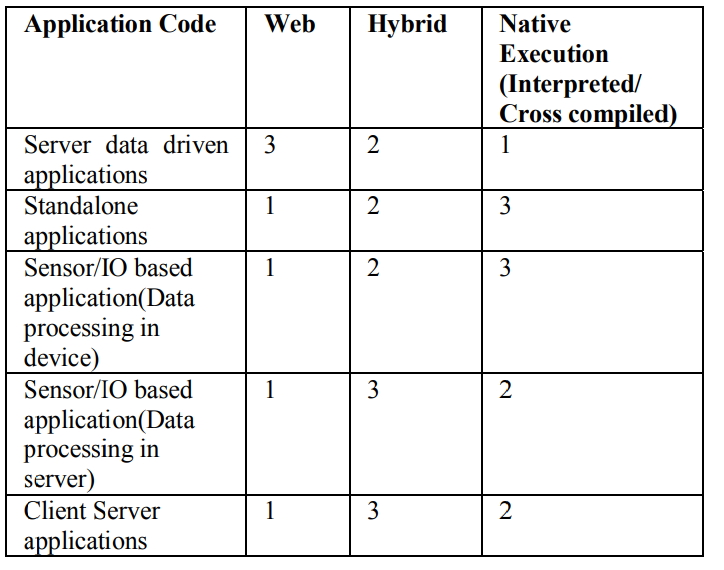
\includegraphics[height=7cm,keepaspectratio]{images/IEEE_related_chapter.jpg} 
  \caption{Entscheidungstabelle für Applikationstyp und bevorzugter Ansatz \cite{IEEE_Rahul_Seshu}}
  \label{fig:decision_table_IEEE_related_work}
\end{figure}

Diese Arbeit stellt einen guten Überblick über einen möglichen Entscheidungsweg dar und erklärt einige wichtige Grundlagen, die zur Unterscheidung bei der Entwicklung von Multi-Plattform-Anwendungen wichtig sind. Jedoch wird einerseits in dieser Arbeit der Aspekt der rein nativen Entwicklung mit den Plattform spezifischen Entwicklungsmethodiken komplett vernachlässigt und die Arbeit stützt sich lediglich auf Recherchen, es wurden jedoch keinerlei Versuche oder messabaren Werte genutzt. Anders ist hier die nächste Arbeit.


\subsubsection{Approaches to mobile application development: Comparative performance analysis - Delia et Al}
Delia et Al vergleichen in ihrer Arbeit die Performance von verschiedenen Ansätzen zur Entwicklung von mobilen Applikationen. Auch sie unterscheiden zunächst, die verschiedenen Klassen der Entwicklungsmethoden. Danach stellen sie ihre Testmethodik vor. Um die Performance der Unterschiedlichen Plattformen zu testen nutzen sie hierfür eine Mathematische Berechnung indem die Summe über 500.000 Schleifendurchläufe einer Berechnung bestehend aus einem Logarithmus, einer Wurzel und Fakultät berechnet wird. Um das ganze etwas differenzierter zu betrachten nutzten sie dafür verschiedene Android und iOS Geräte um die sieben verschiedenen Anwendungen laufen zu lassen. Um die Zeit zu messen, die die Berechnung dauerte, namen sie vor und nach der Ausführung der Berechnung die Zeit und bildeten daraus die Differenz um zu sehen wie lang die jeweiligen Berechnung dauerte. Dies führten sie dann jeweils 30 mal aus und berechneten daraus die Durchschnittliche Laufzeit T und die Standardabweichung S. Das Ergebnis ist in Abbildung \ref{fig:result_table_IEEE_related_work} zu sehen.\cite{IEEE_development_classes}

\begin{figure}[ht]
  \centering
  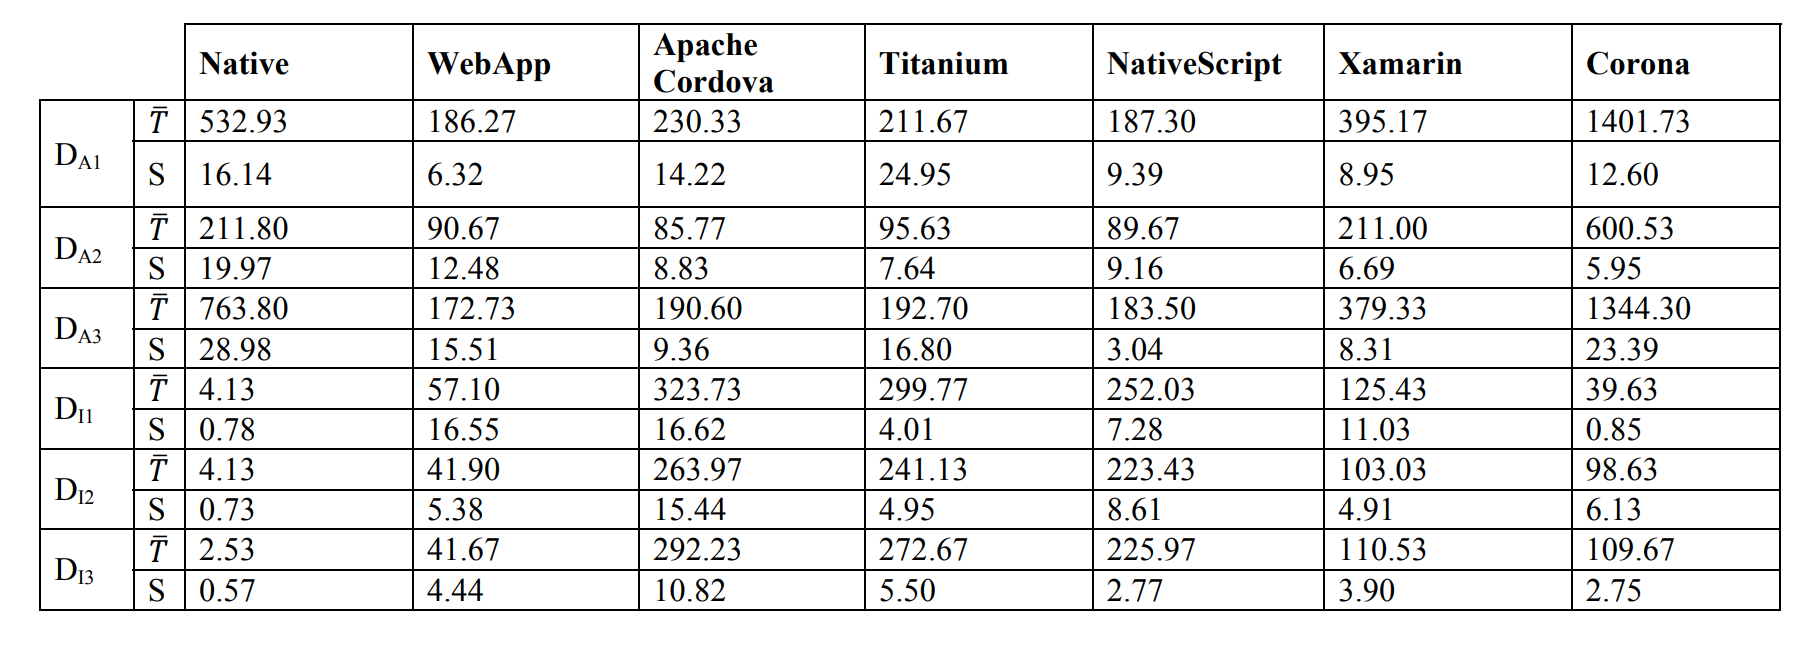
\includegraphics[width=\textwidth,keepaspectratio]{images/IEEE_Delia_Al.png}
  \caption{Ergebnisstabelle der Performancemessungen \cite{IEEE_development_classes}}
  \label{fig:result_table_IEEE_related_work}
\end{figure}

Interessant ist hier vor allem zu sehen, dass es erhebliche Unterschiede zwischen Android und iOS gibt. So ist nicht sichergestellt, dass nur weil ein Ansatz auf Android sehr schnell lief, er auch auf iOS so gut lief. Jedoch erklären sie hierzu selber in der Auswertung ihrer Arbeit, dass ein Vergleich durch die Verwendung verschiedener Hardware schwierig ist.\cite{IEEE_development_classes} Dennoch sagen sie selber, dass die benutzte Implementierung auf iOS effizienter scheint, als die auf Android, was sie auf die Android Runtime zurückführen. Generell stellten sie fest, dass Web-Applikationen in ihren Test die beste Performance über die Geräte hinweg zeigten.\cite{IEEE_development_classes}

In dieser Arbeit wurde lediglich auf die Performance der Applikationen eingegangen. Zu der Webentwicklung gehören jedoch so viel mehr Aspekte, die einen Einfluss auf die Auswahl der Entwicklungsmethode haben. Dazu kommt, dass die Arbeit, da sie 2017 bereits geschrieben wurde, heute komplett anders aussehen könnte/würde. Nicht nur, dass mittlerweile auf beiden Plattformen neue und performantere Programmiersprachen genutzt werden, sondern auch die Geräte von heute haben deutlich schnellere Prozessoren, mehr Arbeitspeicher und vieles mehr. Ein Smartphone von 2017 ist mit einem heutigen nicht mehr vergleichbar. Deswegen rückt der Faktor der Performance immer weiter in den Hintergrun, was auch eine recht neue Untersuchung von 2020 von Bi{\o}rn-Hansen et Al bestätigt. Sie fanden zwar einige Unterschiede zwischen den verschiedenen Frameworks gefunden, kamen aber am Ende zu dem Fazit, dass zwar in der Summe die nativen etwas besser Abschnitten, aber einige hybriden Ansätze in ein paar Aufgaben sogar besser performten als die nativen und kein Ansatz in allen Punkten besser war als die anderen.\cite{BirnHansen.2020}

\subsubsection{Framework Choice Criteria for Mobile Application Development - Khachouch et Al}
Ebenfalls eine neuere Untersuchung ist die folgende von Jhachouch et Al. Ihr Ziel war es dabei einen Entscheidungsgraphen zu erstellen, bei dem man durch Beantwortung einiger Fragen am Ende zu einer Antwort gelangen soll. Sie kritisierten, dass es durchaus einige solcher Graphen gäbe, jedoch dies oft in Richtung eines beworbenen Frameworks manipuliert wären. Deswegen entwickelten sie einen Fragekatalog und Graphen, der keine Aussage zu einem bestimmten Framework oder Technologie einer Firma trifft, sondern dass zu einer Entwicklungsmethodik rät. Das Ergebnis daraus kann man in Abbildung \ref{fig:decision_graph_IEEE_related_work} sehen.\cite{IEEE_Khackouch_Al}

\begin{figure}[ht]
  \centering
  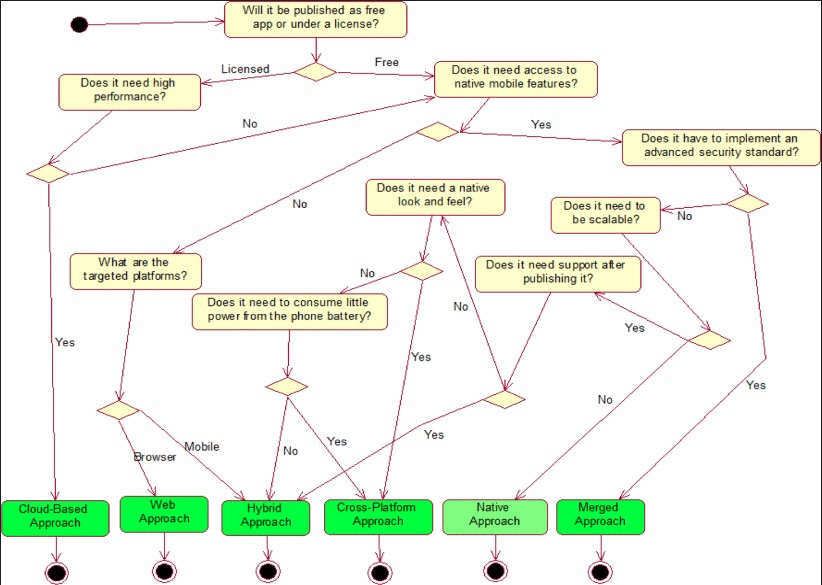
\includegraphics[width=\textwidth,keepaspectratio]{images/IEEE_Khachouch_Decision_Graph.jpg}
  \caption{Entwickelter Entscheidungsgraph von Khachouch et Al \cite{IEEE_Khackouch_Al}}
  \label{fig:decision_graph_IEEE_related_work}
\end{figure}

Sie ziehen am Ende das Fazit, dass wenn "keine Einschränkungen im Bezug auf Kosten oder Personal existieren, der native Ansatz aufgrund seiner Vorteile in Bezug auf Qualität, Leistung und Ergonomie die beste Lösung"\cite{IEEE_Khackouch_Al}{Chapter~4} sei.

Das Problem an dieser Arbeit ist, dass einerseits es in der Realität es nie den Fall geben wird, dass es keine Einschränkungen bei Kosten oder Personal geben wird. Desweiteren ist es auch dann nicht verständlich, warum etwa ein Cross-Plattform Ansatz nicht auch gut sein könnte. Auch die gestellten Fragen und ihre Anworten sind manchmal etwas irritierend. So ist die Frage ob die Anwendung nach einer Veröffentlichung weiterhin Support benötigt. Bei der Antwort Ja wied der Hybride Ansatz empfohlen bei Nein geht es weiter und nach ein bis zwei Fragen wird dann zwischen Hybriden und Cross-Plattform Ansatz entschieden. Jedoch sollte eine App immer weiter unterstützt beziehungsweise gewartet werden. So sollten etwa Sicherheitsupdates von genutzten Bibliotheken oder sonstiges in Apps eingebaut werden können. Auch die Begründung, warum Cross-Plattform Ansätze ein Support nach der Veröffentlichung hier problematisch ist, erklären sie nicht. Sie sagen sogar in ihrer Erläuterung der Fragen, dass alle von ihnen Untersuchten Ansätze einen guten Support anbieten.\cite{IEEE_Khackouch_Al} Ein Argument der hier angebracht werden könnte, ist, dass Cross-Plattformen stark von ihrer Popularität abhängig sind. So können Frameworks eingestellt werden, wenn sie keine aktive Community mehr haben. Jedoch werden selbst dann oft noch durch Open-Source Unterstützer wichtige Updates veröffentlicht um einen Langzeitsupport zu ermöglichen.\TODO{Nochmal überarbeiten. Noch nicht zufrieden.}
\chapter{Grundlagen}
Bevor genauer in die Arbeit eingestiegen werden kann, müssen jedoch erst mal die Ausgangssituation dargestellt, ein paar Begriffe geklärt und das Thema etwas abgesteckt werden.

\section{Projektbeschreibung}
Zu Beginn der Arbeit bestand bereits eine Website, die durch einen internen Workshop konzeptioniert und durch ein Pflichtpraktikum implementiert wurde. Die Website wurde mit der Web-Technologie Elixir gebaut, die sowohl Frontend als auch Backend beinhaltet. Hierbei handelt  es sich um eine Plattform, die das Ziel hat, das Verleihen und Leihen innerhalb von Bekanntschaftskreisen zu vereinfachen/ ermöglichen. Hierfür kann jeder Nutzer seine eigenen, verleihbaren Gegenstände auf der Plattform eintragen. Zusätzlich können Nutzer sogenannte Kreise erstellen und zusammen mit Freunden bzw. Familie beitreten. Jeder kann dann die Gegenstände sehen, die in den verschiedenen Kreisen verfügbar sind, in denen er Mitglied ist. Zur Kontaktaufnahme gibt es ein Chatsystem, bei dem sich Leute Nachrichten hin und her schicken können, um den Austausch zu organisieren.

\section{Funktionsumfang der Beispiel Anwendung}
Grundsätzlich wurde beim Entwurf des Funktionsumfang versucht, die typischen Funktionalitäten von Applikationen abzubilden. Eine Befragung mobiler Anwendungsentwickler durch JetBrains ergab, dass die wichtigsten Funktionen Datenspeicherung, Kommunikation über Netzwerk, Medienanzeige, Status und Navigationsmanagment, Datensynchronisierung, Dateien lesen/schreiben, Sicherheit, Bezahlung, Berechnungen und Machine Learning sind\cite{JetBrains_miscellaneous_2021}. Natürlich sind gerade der letzte Punkt oder die Bezahlung eine sehr Anwendungsfallspezifische Sache, jedoch gibt es einem einen guten Kompass was eine App so grundlegend Abzudecken hat.
Um den Arbeitsaufwand realistisch zu halten und trotzdem aber einige der oben genannten Parameter abzudecken, ist die Implementierung wie im Folgenden beschrieben eingeschränkt:

Allgemein soll eine App gebaut werden, die wie bereits erwähnt sich an einer bestehende Webanwendung orientiert und einen Teil der Funktionalität durch die Programmierung abbilden soll. Des weiteren wird eine GraphQL-Schnittstelle genutzt um die Daten der Webanwendung zu Nutzen. 

\subsection{nativ und Multiplattform v}
Bei der Nativen und der Multi-Plattform Applikation bilden wir den in Abbildung \ref{fig:pageflow} dargestellten Ablauf ab. Dabei sind diese komplett durch in der Applikation implementierten Seiten dargestellt. Diese sind eine Startseite, eine Login- , Profil- , Kommunikations- und einer Chatseite. Dadurch schaffen wir es, die oben genannte Aspekte bis auf Bezahlung und Machine Learning, die für diese Applikation auch kein Anwendungsfall haben, größtenteils abzudecken. Denn durch den Login etwa erfüllt die Applikation teilweise die Bereiche Sicherheit, Statusmanagment, Daten lesen/schreiben und Kommunikation über Netzwerk. 

\begin{figure}[ht]
  \centering
  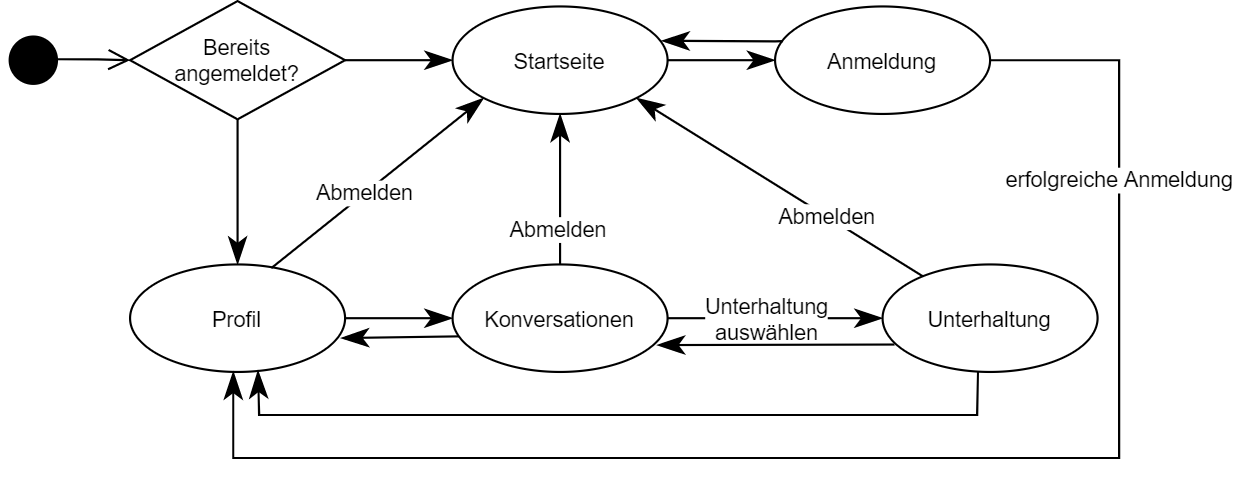
\includegraphics[height=7cm,keepaspectratio]{images/Pageflow_native_flutter.png} 
  \caption{Verbindungen zwischen den Seiten der implementierten Applikation beim nativen Ansatz und dem Multi-Plattform-Ansatz}
  \label{fig:pageflow}
\end{figure}

Der genaue Ablauf der App ist, dass der Nutzer die App öffnet. Ist er beriets eingelogt, wird er automatisch auf die Profil Seite übergeleitet, auf der seine eigenen Sachen angezeigt werden. Ist er nicht angemeldet, so landet er auf einer Startseite/ Willkommensseite, auf der einige Sachen über das Projekt erklärt werden und kann dann zu der Loginseite weiter, von der er nach erfolgreichem Anmelden zu der bereits erwähnten Profilseite kommt. Über einen Knopf in der Menüleiste der App kann der eingeloggte Nutzer auf die Konversationsseite wechseln. Hier wird im eine Liste an Konversationen angezeigt, an denen er beteiligt ist. Nun kann er durch einen Klick auf eine Unterhaltung zu dem Chat wechseln, kann hier die bereits bestehenden Nachrichten lesen und neue Nachrichten abschicken. Mit der Zurück-Taste kann er dann wieder zu der Konversationsseite zurückkehren oder über einen Klick auf das Logo zur Profilseite zurückkehren. Als letztes ist in der Menüleiste noch ein Knopf mit dem Text "Abmelden". Wenn man diesen drückt, werden die gespeicherten Zugangsdaten gelöscht und der Nutzer somit abgemeldet. Nach erfolgreichem Abmelden wird er dann wieder zu der Startseite zurückgeführt.

\subsection{hybrider Ansatz und Mix Ansatz}
Bei den hybriden Absätzen wird die Website mit in die Applikation eingebunden. Je nach Art des hybriden Ansatzes unterscheidet sich hier der Umfang und Ablauf. So wird etwa bei den in Kapitel 4.2 vorgestellten Implementierungen unter Umständen nur die Website in einer Applikation angezeigt. In Kapitel 4.4 jedoch wird die oben erklärte Implementierung mit einer Anzeige der Website gemischt. So wird im vergleich zu Abbildung \ref{fig:pageflow} die Startseite durch die Startseite der Webseite ersetzt. Zusätzlich dazu wird durch eine veränderte Navigation über ein Seitenmenü die zusätzliche durch die Webanwendung verfügbare Funktionalität durch Verlinkung hinzugefügt. Etwa kommen hierdurch eine Übersicht der Kreise in denen der Nutzer Mitglied ist oder eine Liste der Gegenstände die man ausleihen kann hinzu.

\section{Themenabgrenzung}
In der Arbeit werden die Implementierungen auf eine Android Implementierung beschränkt, insofern sie nicht durch das Framework automatisch mitgeliefert werden. Das hat zwei Hauptgründe. Einerseits um den Aufwand für die Implementierung zu beschränken und andererseits sind iOS und Android insofern vergleichbar, da beide nativ auf die vollständigen Funktionalitäten der Betriebssysteme zugreifen. Außerdem sind es nicht die verschiedenen Programmiersprachen und ihre Kleinigkeiten die entscheidend sind, um native Apps zu entwickeln, sondern die Konzepte. So sagen Goadrich et Al in einer Untersuchung, welche Plattform für einen Universitätskurs passend wäre, dass etwa beide Umgebungen fähig sind sowohl 2D als auch 3D Graphiken mit OpenGL und Datenbanken und ihr Managment mit SQLite zu erzeugen.\cite{iOSvsAndroid}Weiter sagten sie, dass Studenten praktische Beispiele von integrierten Betriebssystem sehen könnten und lernen würden mit Threading, Synchronisierung und Locking umzugehen\cite{iOSvsAndroid}. Sie kommen am Ende auf den Schluss, dass es wegen diesem und anderem, kein Unterschied macht welche Plattformumgebung genau gelehrt wird und dass eine Programmierung, mit egal welchem, helfen würde, die Grundideen der mobilen Programmierung zu vermitteln. \cite{iOSvsAndroid}
Natürlich gibt es kleinere und größere Unterschiede zwischen den Programmiersprachen und der Implementierung auf den Plattformen, aber die Nutzung der Betriebssystemspezifischen Schnittstellen und die dahinter liegen Konzepte sind grundlegend gleich.
\TODO{Kein wörtliches Zitat. Übersetzt und nur Sinn mäßig und Ende vervollständigen}

Des weiteren wird in dieser Arbeit eine Möglichkeit der Spieleimplementierung nicht betrachtet. Diese stellen zwar immerhin einen großen Teil der in den Appstores vorhandenen Anwendungen dar, Jedoch sind dies keine typischen Apps die von Appagenturen oder privaten Entwicklern produziert werden, sondern eher von Unternehmen mit Grafikentwicklungs- oder Spieleentwicklungshintergrund. Außerdem werden die meisten Apps nicht in Kotlin oder Swift direkt entwickelt sondern mit Game- und Grafik Engines. Zwar gibt es auch Ansätze, wie Flutter Flame, eine Libary die helfen soll, 2D Games mit Flutter zu entwickeln, 
\TODO{Schlusssatz}
\TODO{Quellen}

\section{Begriffe}
wda
\TODO{Hier noch Sachen umstellen, hinzufügen, und eventuell an Start des Kapitels stellen}
Wenn in dieser Arbeit von einer App oder Applikation geredet wird, so ist hiermit eine Anwendung gemeint, die für mobile Endgeräte, vor allem Smartphones mit den Betriebssystemen Android beziehungsweise iOS gebaut wurden.

Außerdem ist in dieser Arbeit oft die Rede von Multi-Plattform-Anwendungen. Darunter versteht man eine Anwendung, die nicht nur für eine Plattform geschrieben wurde, sondern für mehrere. Dies beinhaltet dann beispielsweise die verschiedenen Smartphone Plattformen, oder aber auch die verschiedenen PC Plattformen wie Linux oder MacOS. Eine Anwendung muss dabei auch nicht alle Plattformen beinhalten, sonder kann auch nur zwei abdecken. Statt Multi-Plattform-Anwendungen wird häufig auch Cross-Plattform-Applikationen als Begriff genutzt, da dies ein in der Industrie häufig benutztes Synonoym ist. 

\section{Die verschiedenen App Development Framework Klassen}
Wenn man über Applikationsentwicklung für mobile Endgeräte spricht, muss man zwischen \TODO{genaue Zahl einfügen} verschiedenen Varianten unterscheiden.
\subsection{Native Applikationen}
Native Apps sind Applikationen die entwickelt werden um auf einer spezifischen Plattform, abhängig des Gerätetyps, des Betriebssystems und der Version zu laufen. Der Quellcode wird dafür zu ausführbaren Code übersetzt.\cite{IEEE_development_classes}
Das bedeutet, dass etwas um eine native Android App zu erstellen, wird diese etwa in Kotlin, die Plattform typische Programmiersprache, programmiert und im Anschluss in Bytecode übersetzt.

Der Vorteil der nativen Entwicklung ist, dass man die Funktionen der verschiedenen Plattform optimal ausnutzen kann. So ist etwa eine Nutzung der Kamera, GPS, Beschleunigungssensoren, Kalender und vielem mehr denkbar einfach. Es gibt eindeutig definierte Schnitstellen und diese müssen nur aufgerufen werden. Dabei ist die Ausführung nicht nur schnell sondern kann auch einfach im Hintergrund ausgeführt werden. Auch eine Benachrichtigung des Nutzers ist problemlos möglich, da man einfach die Schnittstellen der Plattform nutzen kann. Außerdem funktionieren sie, mit eventueller Funktionseinschränkung, auch ohne, dass der Nutzer mit dem Internet verbunden ist. \cite{IEEE_development_classes}

Ein weiterer Vorteil ist, dass man die volle Kontrolle über das Aussehen und der Funktionsweise innerhalb der Plattformgrenzen hat. So kann man dass man vollständig angepasste Nutzeroberflächen bauen, die auf die mobile Plattform aber vor allem an die eigene App angepasst sind. Man ist dadurch nicht abhängig von den Funktionsmöglichkeiten möglicher Zwischenschichten.

Einer der größten Nachteile der nativen Entwicklung jedoch ist der Aufwand und die damit verbundenen Kosten, um für die verschiedenen Plattformen eine Applikation anbieten zu können. Denn die Applikation muss größtenteils für jede Plattform komplett neu gebaut werden. Doch nicht nur die Programmierung ist ein Kostenfaktor. So nennt Delia et Al als weitere Faktoren das Testen, Wartung und Verteilen neuer Version als weitere Faktoren, die auf jeder einzelnen unterstützten Plattform auftreten.\cite{IEEE_development_classes} Dazu kommt, dass man für jede Plattform auch Entwickler benötigt, da sich die wenigsten Entwickler auf allen Plattformen auskennen und Anwendungen für die verschiedenen Plattformen oft auch gleichzeitig entwickelt werden sollen. Dadurch werden aus Anwendungen die auf mehreren Plattformen veröffentlicht werden, schnell große Kostenproduzenten. Deswegen werden hier oft bei kleineren Anwendungen die Implementierung auf eine oder zwei Plattformen beschränkt, was die Reichweite der App vermindert.

\subsection{Web Applikationen}
Web Applikationen sind Applikationen, die einfach nur im Netz verfügbar sind. Sie sind darauf ausgelegt, als Webseiten auf einem Server zu laufen und dann über den Browser der Geräte aufgerufen zu werden. Dieser Ansatz ist denkbar einfach, da bereits einfachste Seite sofort für jeden Nutzer verfügbar sind, sobald sie auf dem Server gestartet wurden. Sie müssen auch nur lediglich einmal entwickelt werden, da sie auf allen Geräten mit einem Browser und einer Internetverbindung aufgerufen werden können. So kann man alle Plattformen mit nur einem Code abdecken.\cite{IEEE_development_classes}

Dennoch hat man hier große Einschränkungen, da sie lediglich die Funktionalitäten zur Verfügung haben, die der Browser anbietet. So können die nativen Schnittstellen nicht genutzt werden und sind in ihrer Funktionalität stark beschränkt. Dazu kommt, dass wenn keine Internetverbindung vorhanden ist, die Anwendung gar nicht genutzt werden kann und bei einer langsamen Internetverbindung die Performance signifikant sinkt. 

Diese Klasse wird jedoch in dieser Arbeit nicht behandelt, da hier auf Anwendungen konzentriert wird, die sich auf einem Gerät installieren lassen und somit als Programme auf dem Gerät verfügbar sind.

\subsection{Hybride Applikationen}
Eine Klasse die dafür durchaus in der Arbeit untersucht wird ist die der hybriden Apps. Diese sind Applikationen die zu einem Teil aus nativem Code besteht und zu einem anderen Teil aus einem Web-Container. Sie benutzen also Web-Technologien, benutzen aber nicht den Browser, sondern einen Web-Container. Unter Umständen kann dieser mit Hilfe von bestimmten API-Schnittstellen auf Gerätespezifische Funktionen zugreifen.\cite{IEEE_development_classes}


\subsection{Cross Plattform Applikationen}
3. Cross-Plattform-Apps
Unterscheidung zwischen Webview in App und z.B. Flutter 

\chapter{Entwicklung}
Im 4. Kapitel dieser Arbeit sollen nun verschiedene Implementierungen und Ansätze erklärt und erläutert werden, Darauf sollen auf Herausforderungen eingegangen werden und ein kurzes Fazit zu den verschiedenen Ansätzen gezogen werden. Dabei wird jeweils nur auf eine Android Implementierung eingegangen. 
\section{Entwicklung Nativer Android Applikation}
Als erste Implemetierung soll nun die native Android Applikation vorgestellt werden. Wie bereits in der Abgrenzung erwähnt, beschränkt sich diese Arbeit auf eine Android Implementierung, um einerseits den Aufwand zu begrenzen und da es wie bereits aufgezeigt native Implementierungen grundsätzlich vergleichen lassen, da diese direkt auf die meist auf beiden Plattformen vorhandenen spezifischen Schnittstellen zugreifen. Außerdem sind die grundsätzlichen Entwicklungskonzepte die gleichen und lediglich die Feinheiten der Programmiersprache unterscheiden sie.

\subsection{Grundlagen}
Solange es Smartphones gibt, gibt es auch schon die native Entwicklung. Android etwa wurde 2008 vorgestellt. Damals wurden die Apps in Java entwickelt, eine Sprache die in der Anwendungsentwicklung damals und heute noch sehr gut bekannt ist und auch oft noch als Programmiersprachen an den Universitäten gelehrt wird. 2019 jedoch änderte Google die offiziell bevorzugte Programmiersprache zu Kotlin. Kotlin wurde von Jetbrains entwickelt um einen Ersatz für Java zu finden, dass alle benötigten Funktionen für eine effektive Appentwicklung hat, jedoch genauso schnell kompiliert werden kann. Mittlerweile ist es nichtmehr nur noch die bevorzugte Sprache von Google, sondern auch von den Entwicklern. //Kotlin Apple ihre ersten Applikationen für iOS mit Objectiv-C programmiert. Beide Arten werden auch weiterhin unterstützt. Jedoch gibt es mittlerweile Programmiersprachen, die speziell an die Bedürfnisse der Betriebssysteme angepasst sind und deren Entwicklung die Firmen selbst vollständig in der Hand haben, um schnell und Unkompliziert benötigte Änderungen vornehmen zu können. So empfiehlt Apple mittlerweile Swift und Android die Verwendung von Kotlin.

 So ist Kotlin eine auf Java basierende Programmiersprache die bidirektional übersetzt werden kann. So kann man alten Java Code in die Kotlin App einbinden und automatisch übersetzen lassen. Außerdem wird der Kotlin Code zum bauen der App in Java übersetzt und dann in Java ausgeführt.
Nachdem dies aus dem Weg geschafft ist und wir uns also für Kotlin in diesem Fall entschieden haben, gibt es nun weitere Entscheidungen zu treffen. Bei Android Apps kann man grundsätzlich zwischen zwei verschiedenen Arten des Seitenaufbaus und der Grundarchitektur. 
Diese nennen sich Activitys bzw. Fragments. Sie sind die Entscheidung für eine Art Grundstruktur. Bei Activitys sind die einzelnen Seiten unterschiedliche Klassen und eigenständige Systeme. Jede Activity hat ihren eigenen Context und wird selbständig auf dem Bisldschirm aufgebaut. Danach wird neben ein paar ausnahmen nur zwischen den eigenen Activitys hin und her navigiert um den Ablauf der App nachzubilden.
Bei Fragments haben diese einen geteilten Kontext. Sie werden alle gleichzeitig gebaut und werden dann nur darübergelegt bzw. vom Bildschirm entfernt. Ein großer Vorteil dieser Methode ist, dass man wenn man genügend Platz hat, zwei Bildschirme nebeneinander angezeigt werden können und diese beide normal funktionieren. Bei kleinen Bildschirmen oder unter Umständen kann auch dann nur ein Fragment angezeigt werden. Somit zeigt sich, dass vorallem für Anwendungen die sowohl auf Tablet und Handy Problemlos genutzt werden sollen, Fragments sich gut eignen.
Beide Ansätze haben ihre Vor- und Nachteile.
Für diese Arbeit wurde entschieden auf die Activitys Architektur zurück zu greifen, da sie anfänglich einfacher ist und Schwierigkeiten mit dem Kontextmanagment und dem App Backstack zum navigieren durch die History reibungsloser funktioniert. Außerdem sind Activities aktuell besser dokumentiert und viele Problemlösungen sind für Activities beschrieben.

Nach dem man sich nun für eine Grundarchitektur entschieden hat, müssen ein paar Entscheidungen anhand der Projektarchitektur getroffen werden. Ersteinmal muss man entscheiden ob man eine lokale Offline Datenbank braucht oder ob man eine Onlinedatenhaltung mit eventuell angebundener Serverlogik hat. Natürlich kann auch beides gemacht werden. Jedoch in diesem Fall werden wir nur eine Onlinedatenhaltung benutzen die über eine API angebunden ist. 


Ärgerlich bei der Nativ Entwicklung und Graphql war, dass neu erzeugte Querys erst durch ein Build durchlauf erzeugt wurden, und so etwas längert braucht zur Entwicklung.

\subsection{Schwierigkeiten}
\subsection{genutzte externe Bibliotheken}
\subsection{Fazit Nativ}
\section{Entwicklung Hybrider Android Applikation mit WebView}
Es gibt noch einen anderen Weg eine Anwendung auf mehrere Plattforment zu bringen.
Und zwar eine Website in einer nativen App anzuzeigen. So muss man lediglich eine Website schreiben die auch gut auf verschiedenen Bildschirmgrößen angezeigt werden kann. Danach muss man nur noch ein paar Anpassungen an einer nativen Android App vornehmen, um eine Reibungslose funktionalität zu gewährleisten und schon hat man eine Applikation die als Website auf allen Geräten aufgerufen werden kann und man kann sie gleichzeitig noch in eine Webview einbauen, um seinen Nutzern eine Appversion bieten zu können, die diese aus den Appstores herunterladen können.
\subsection{Abstufungen}
Diese Entwicklung kann jedoch noch generell in zwei unterschiedliche Abstufungen unterteilt werden. 
\subsubsection{Reine Webview ohne nativen Anteil}
Hier wird nur die Website auf einem "Canvas" angezeigt und noch ein paar Konfigurationen vorgenommen, damit alle Funktionalität grundsätzlich angeboten werden kann.

\subsubsection{Webview gemischt mit Nativer Funktionalität}
Es gibt Optionen einen Nativen anteil in eine WebView App einzubauen.
\subsubsection{Einbau des Android Adapters in Website um native Funktionalität aufzurufen}
Neben der einfachen WebView kann man wenn die Website Javascript benutzt auch native Funktionalität einbauen. So kann man eine Javascript Verbindung erstellen indem man im Javascript der Website eine Android Adapter aufruft und dort eine Funktion aufruft, die im Android Code definiert ist. So kann man native Funktionalität auf Smartphones nutzen.(Toast beispiel)
\subsubsection{Mischen zwischen Nativer und Webansicht}
Einen Schritt weiter als davor. Hier schreibt man die Website bereits in einer passenden Technologie/ Sprache, um im Anschluss eine App zu entwickeln, die native und Web Ansichten mischt, um einen möglichst effizienten aber trotzdem nativ aussehenden Look für eine App zu erhalten. Hotwire und Turbo. als Beispiel
Diese Technologie wurde von der Firma Basecamp entwickelt, die schon lange für ihre Plattform eine schnelle Lösung für ihre Websiten gesucht haben. Daher haben sie Hotwire erfunden. Hotwire steht für HTML over Wire. Was das bedeuted ist, dass die Website nicht andauernd komplett neugeladen wird, sondern nur die teile, die auch erneuert werden müssen. Dazu kommt noch einige technologie die das caching und die verarbeitung der benötigten javascript Files handelt und raus kam eine Lösung um schnell und performant Websiten zu laden.
Um das ganze nun auf ein Smartphone zu bringen war die Idee entsanden, dass man hier nicht eine komplette native App schreiben wollte sondern eben eine WebView herzunehmen, in die aber Native Teile gemischt weren, um die Erfahrung der Nutzer möglichst intuitiv zu gestalten. 



\subsection{Fazit(muss wsl. wo anders hin) zu hybrid}
Auch wenn es auf dem ersten Moment super einfach scheint und es so wirkt, als könnte man so jede Website einfach in eine Applikation stecken, ohne dass man groß wiederholenden Code hat, bzw. dass man mehrmals die komplette Anwendung schreiben muss, sondern ja nur einmal und je nach grad noch einmal Aufwand hineinstecken muss, aber nie in dem Umfang wie für eine komplette native App. 
Es hat auch Nachteile und Gründe, warum dies nicht gern genutzt wird.
Ein aller erster großer Nachteil ist eine reine online Funktionalität. 
\section{Entwicklung Cross-Plattform Applikation mit Flutter}
Notizen zur Entwicklung mit Flutter:
\TODO{https://www.youtube.com/watch?v=wE7khGHVkYY}
Composition: Composing different existing widgets to a new one

Durch voreinstellung und Erstellen eines Basic screen schon nach wenigen Minuten eine erste laufende "Version" zu sehen.

Hot Reload zeigt sofort sichtbare Änderungen, so dass man gut UI debuggen umbauen und anpassen kann.

Schwer herauszufinden welche Elemente es gibt, wie man sachen konfigurieren kann. Am Anfang nicht sehr intuitiv. Man muss sich auf jeden Fall gut in die Doku einlesen und vlt. auch ein kleines Tutorial machen, bzw. die genauen Sachen googlen.



\subsection{Flutter 101}
\subsubsection{Widgets}
Widgets sind die Elemente in Flutter, die genutzt werden um die Applikation aufzubauen.
Es gibt zwei Arten von Widgets:
1. Statefull Widget
2. Stateless Widget
Der Unterschied ist, dass bei Statefull widgets, gibt es noch eine State Klasse, die den aktuellen Status des Elements speichert und bei einer Änderung die neuen Werte übernimmt und damit eine Änderung in dem Element ausführt. Am besten ist dies etwa mit einem Favoriten Button vorstellbar. Drückt man ihn, fügt man ihn zu den eigenen Favoriten hinzu und das Icon des Buttons ändert sich bspw. von einem Herzicon, das nur den Rahmen hat, zu einem was ausgefüllt ist.

Bei der Erstellung gibt es einiges zu beachten. 
Etwa kann man auch ein Widget erstellen wollen, dass in ein eigenes File auslagern, wie es mit tobBar.dart ist. Hier ist jedoch dann die übergabe von Parametern wieder wie bei normalen Klassen übergeben werden. Man kann sie aber auch erstellen wie bei topBar2.dart, wo man die einzelnen Parameter bennenen kann und auch besser nullabillity handln kann.
\TODO{genauer untersuchen. Vorallem Statless Widgets, nullability wie bei topBar, und vieles mehr}

Man kann aber auf jeden Fall sehr einfach ein eigenes Widget schreiben. Dies ist vorallem sinvoll, wenn man eine Komponente hat, die man wiederverwenden möchte. Man erstellt einfach die Widgetclasse mit den entsprechenden 
\subsubsection{Plugins, Modules, Packages}
Im Verlauf der Arbeit wurde ebenfalls Testweise ein eigenes Plugin geschrieben um zu testen wie hier der entsprechende Ablauf ist, und wie hiermit eventuelle nicht vorhandene Funktionalität mit nativen Programmiersprachen und API calls programmiert werden kann. Hierzu wurde einmal die Einführung von der google developer seite TODO: Link genutzt um ein iOS und Android keyboard zu schreiben das auf dem Gerät anhand von nativen APIs der Betriebssysteme die Töne erzeugt und dabei sowohl auf drauf drücken und loslassen reagiert.
Das interessante an dieser Methode ist es , dass zur Kommunikation zwischen dem Dart Code und dem nativen Code channels zur Kommunikation genutzt werden, um dann die entsprechende native Funktionalität auszuführen. Ein zweiter interessanter Punkt ist, dass plugins asynchron auf eigenen Threads ausgeführt werden/können. Dies folgt der größeren Diurektive dass UI und Logik auf unterschiedlichen Threads laufen, um mögliche Blockaden nicht auf dem jeweils anderen Thread bem,erkbar zu machen.



\subsubsection{Layout}
-Button
-Row
-Wrap
-Container: Dies ist das Wichtigste Widget von Flutter. Sobald man irgendwelche Platzhalter oder innere Abordnung oder sonst was nötig ist, braucht man oftmals das Widget Container. Man kann ganz einfach andere Elemente in ein Container hineinstecken und alle benötigten Sachen hinzufügen. Von Margin Paddings feste Größen und vieles mehr. Einfach Einen Container erstelle und die innenliegenden Elemente in einem ChildWidget hinzufügen.
-Scaffold
\subsubsection{Aufbau}
-Widgets
-classes
-Stateclasses
-Navigator / Router
-Assets

\subsubsection{Plugins / pubspec.yaml}
\subsubsection{benutzte Plugins}
\subsubsection{Lehre aus Unterhaltung mit Entwicklern von Plugins}
Bei erstellen erster Seiten und hinzufügen ersten Packages Fehler aufgetreten betreffend Not implemented. Fehlermeldung und Fehler-stack nicht sehr aussagekräftig. Wurde evaluiert dass es an simple gradient text lag. Laut Dokumentationseite des Packages ist es kompatibel für alle Plattformen. Jedoch funtkionierte es nach hinzufügen der Vorgeschlagenen Lösung nur noch auf Android/mobile. Beim Nachforschen tut man sich schwer genaue Gründe herraus zu finden, da die Fehlermeldung und die Dokumentation hierfür leider keinerlei Hinweise gibt. 
Es kam im Verlaufe der Fehlererforschung auch zum Kontakt mit dem Entwickler der sehr hilfsbereit die Fehlerforschung unterstütze.
\TODO{Ergebniss der Issueunterhaltung mit Entwickler}
Bei genauer untersuchung mit dem Entwickler zusammen kam herraus, dass meine Flutterversion eine ältere war, als die, die benötigt wurde, um das Plugin auf Web laufen zu lassen. Nachdem die Flutter version angepasst war, funktionierte es einwandfrei. Da es jedoch bei vielen Packages und auch bei diesem keine Angaben zur mindestens zu nutzenden Flutterversion gab, empfohl ich dem Entwickler doch dies in der Read.me hinzuzufügen, was auch prompt geschah. 
An diesem Beispiel sieht man sehr gut, dass diese Community sehr aktiv und offen ist für Vorschläge und Veränderungen.
Es hat mir jedoch auch gezeigt, dass einige Sachen hier Fehlen:
1. Eine Angabe welche Flutterversion genutzt werden muss, damit alles gut funktioniert. Es gibt zwar eine Angabe unter welcher Version das Plugin getestet wurde, aber manchmal will man vlt. gar nicht sofort auf die neueste Version wechseln.
2. Eine Anzeige welche Packete und Flutterversionen geupgraded werden können, fehlen. Es muss irgendein Anhaltspunkt geben um schnell zu sehen, welche Plugins bzw. Dependencies veraltet sind und was hier geupdated werden kann.


\subsection{Layouting in Flutter}
SpacerFürTODO
\TODO{Eigentlich hat ja android das auch. Hier sind halt die Layout Files wirklich nur } 
\TODO{reine Layout Files aber sie sind ja auch xml. Siehe vergleich mit HTML+CSS} 
Flutter ist ersteinmal etwas anderes als die native Entwicklung. 
\TODO{Mit iOS abgleichen}
Containerisierter Aufbau Abgleich miut Kapitel zu Layout aus der Flutter - Doku

Flutter ist ähnlich zu html+css Aufbau Man verschachtelt die verschiedenen Elemente ineinander um dann einen Container-Baum zu erhalten.
Dies ist sehr ähnlich zum html baum. Der entsteht wenn man eine Website entwirft und die verschiedenen Elemente verschachtelt. 
Allerdings kommt hier auch gleich noch css mit rein, da man die verschiedenen Attribute der Elemeente direkt beschreibt.
Was anders ist, ist dass man für Layout spezifische Sachen manchmal noch einen Container braucht, während man ja etwa margin auf jedes Element drauf machen kann. Es ist aber dementsprechend auch wieder ähnlich, da etwa flex boxen manchmal in sogenannte divs eingebaut werden müssen, um zu funtktionieren. Was außerdem besonders ist, ist dass es schon sehr vordefinierte Plugins gibt, die das Layout vorgeben können. Einerseits gibt es rows und Columns, die ansonsten oft über divs mit bestimmten Klassen und Frontend UI Framewortks erreichrt werden können und es gibt oft auch schon spezifizierte Sachen für Buttons etwa. Hier kann man dann OutlinedButton, Button, TextButton oder auch IconButton nehmen um das Design hierfür nicht erst selber bauen zu müssen.

\begin{figure}[ht]
  \centering
  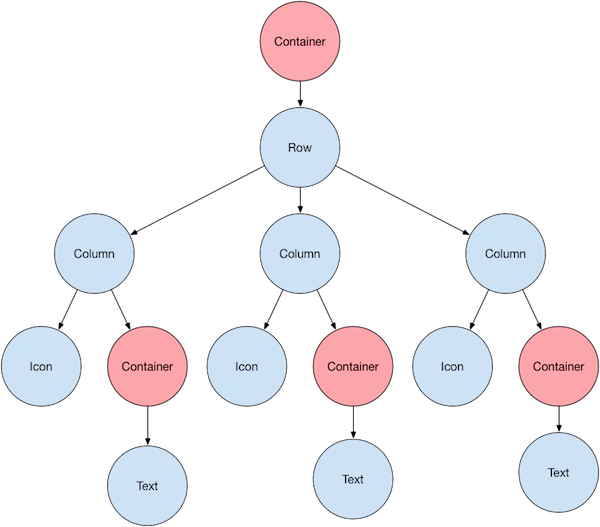
\includegraphics[height=7cm,keepaspectratio]{images/sample-flutter-layout.png} 
  \caption{Hierachie einer Menüleiste Quelle: Flutter Doku}
  \label{fig:flutter_layout_tree}
\end{figure}

Abbildung \ref{fig:flutter_layout_tree}

Um Seiten zu erstellen gibt es verschiedene Methoden. Oft muss man die Seiten komplett selbst aufbauen. Das heißt man fängt beim Startelement an. Dem sogennanten Scaffold. Dieser hat verschiedene Elemente. So gibt es AppBar man kann einen Footer hinzufügen und vorallem gibt es einen Body. Der kann dann ein Widget als Child hinzugefügt werden. Hier kann nun über verschiedene Widgets wieder neue Sachen hinzugefügt werden und so Stück für Stück ein Layout gebaut werden. 
Hierfür gibt es Grundsätzlich zwei verschiedene Arten von Widgets. 
1. Widgets die Helfen die Seite zu strukturieren und Layouts zu verfeinern und aufzubauen.
2. Widgets die Teil der Nutzeroberfläche sind und die unter Umständen noch weitere Childs zur ausgestaltung Besitzen, aber auf der Oberfläche angezeigt werden. So hat etwa ein TextButton noch ein Child Text wo dann der Text hinzugefügt wird, der im Button steht. Der Button ist allerdings ebenfalls ein Teil der UI. Anders als Container. Diese fügen eventuell eine Margin, also Abstand zu anderen Elementen hinzu oder ändern\TODO{Tun sie das wirklich?} unter Umständen auch mal den Hintergrund, sie sind allerdings keine Alleinstehenden Elemente und umgeben eigentlich nur das Child oder die Child Elemente.




\subsection{Conclusion Flutter}
Hier auf die Challanges mit Null safety und grundsätzlichen Änderungen zwischen den großen Versionen eingehen, die dazu führen, dass nicht nur unter anderem auch eigene Dokumentation und Codelabs Einträge nicht mehr funktionieren, sondern auch ein großteil der bestehenden Lösungen so nicht mehr einfach Copy Paste mäßig in die eigene Applikation gezogen werden kann.
Dazu kommt, dass etwa reihenweiße Packages mit einem Update auf Flutter 3.0 wieder ein Update brauchen da hier wieder einige Sachen zu Nullsafety usw. siehe Screenshot mit Warnung aus Console und der Nutzer dann immer eine Warning bekommt, die er so schnell nicht ändern kann. Dazu kommt, dass das upgraden der Dependencys wie bei allen anderem aber auch, wieder zu häufigen Koabhängigkeiten und Upgrade Issues führt, sodass man immer genau aufpassen muss, ob man denn jetzt eine ältere bzw. neuere Version der Plugins nutzen kann. Deswegen gilt auch hier wie in vielem anderen. Versuche so viel wie möglich selbst zu machen. Hierzu vlt. aus dem Artikel zietieren mit jeder Import ist ein "Dept" und irgendwann muss man dann seine Schulden zurückzahlen. Natürlich gilt. Nur so viel wie sinnvoll. Denn man sollte bereits verfügbare Lösungen zu komplexen Problemen schon nutzen, um nicht unnötig Zeit zu verschwenden. jedoch sollte man hier darauf achten, dass man vlt. nur so viel importiert wie nötig ist, um möglich Cropssdependencie errors zu vermeiden.
Ein weiterer Punkt ist die verfügbarkeit auf Plattformen. Nachdem mit Flutter 3 die Lücke der letzten Fehlenden Plattformen geschlossen wurde, heißt es nicht dass man jetzt einfach seine für Android und iOS entwickelte App nehmen kann und dann eine Plattform hinzufügen und dann der Meinung sein dass alles einfach funktioniert. Denn einige Plugins sind nur für bestimmte Plattformen geschrieben. So etwa das WebView Plugin für Flutter. Die populärste von Flutter "promoted(noch mal nachschauen)" Version ist nur für Android und iOS. Das ist ja eigentlich auch erst mal ok, da man ja bei allen anderne Versionen einfach eine Website aufrufen kann und dabei auch keine Layout probleme haben sollte. Aber wenn man sich vornimmt nun für eine andere PLattform eine App mit WebView zu bauen, so hat man leider nie das alles in einem Paket. So gibt es Plugins die unterstützen dann zusätzlich noch Windows Version oder die Webversion, oder eine andere die alle Laptop Plattformen (Mac, Linux, Windows) unterstützt, aber dann wieder nciht die Smatrphone Versionen. Hier muss man also bei Projektbeginn sich überlegen, für welche Plattformen man etwas entwickeln will, bzw. welche Plattformen man ausschließen kann und dann dementsprechen deine Plugins suchen, was eiunen auch stark einschränken kann. Natürlich gibt es jetzt die Möglichkeit einfach sein eigenes Plugin zu schreiben und dabei alle Plattformen zu unterstützen. Dafür muss man sich jedoch dann auch in jeder zu unterstützenden Plattformtypischen Programmiersprache auskennen.

\subsection{Exkurs: Firebase}
Ein weiterer Aspekt, warum Flutter gerade bei kleineren App-Projekten gern genutzt wird ist die vollumfängliche Integrationsmöglichkeit von Firebase. Firebase ist eine Backend-as-a-service (BaaS) Lösung, die dabei helfen soll noch schneller und einfacher Anwendungen zu veröffentlichen. Es sind Produkte und Lösungen auf die man sich verlassen kann, während man seine App entwickelt.\cite{firebase_documentation}

Firebase ist eine Sammlung von verschiedensten Tools und Plugins, die einem Entwickler die Möglichkeit geben soll, eine Applikation zu schreiben, ohne sich groß Gedanken um ein Backend Gedanken machen zu müssen. Es umfasst Tools wie Analytics um Nutzungsdaten zu sammeln, ein fertiges Chatsystem oder auch eine umfangreiche Cloud gestützte Datenbank Lösung. So schreiben Guzzi et Al, dass man ein Developerteam anstellen könnte, das in monatelanger Arbeit ein Backend System programmieren könnte, dass sich mit einer Reihe von APIs zu einer Datenbank verbindet. Man könnte ja aber auch einfach ein bereits bestehendes System nehmen. Mit Firebase muss man nicht mehr tausende Zeilen Code schreiben, um über asynchrone Aufrufe und nebenläufige Prozesse eine reaktive App zu schreiben. Sondern durch Firebase erreicht man das in kürzester Zeit.\cite[p.~608]{Flutter_Apprentice}

Um eine Datenbank für seine App zu erstellen sind es wenige Schritte. So geht man auf die Firebase Website, legt eine neue Datenbank an, danach gibt man seine App-Id die ähnlich zu com.google.chrome ist und kann dann die jeweiligen Konfigurationsdateien für die Plattformen herunterladen. Danach fügt man diese nur noch den einzelnen Plattformen hinzu und kann dann mit der Datenstruktur lokal in der Flutter App entwerfen. Dafür muss man lediglich die Daten-klasse mit JSON Konvertierungen, ein Data-Access-Object (DAO) mit einer Methode zum speichern und holen der Daten und zuletzt noch einen Provider erzeugen. In die drei Datein werden noch die jeweiligen Imports hinzugefügt und schon hat man eine Verbindung zu Datenbank und kann seine Daten in der Datenbank speichern. Ein großer Vorteil, mit der richtigen Konfiguration erhält man gleichzeitig eine offline Datenbak, um so seiner App eine offline Funktionalität hinzuzufügen.\cite{Flutter_Apprentice}

Ein weiterer Pluspunkt ist hier die Integration von Firebase-Authentifizierung. Dadurch erhält man nicht nur automatisch einen Login mit der Möglichkeit, Benutzer zu kategorisieren beziehungsweise die Nutzung einzuschränken. So kann man über Regeln in der Firebase-Website, einen autorisierte Datenzugriff gewährleisten. Ebenfalls kann man so sicherstellen, dass der Nutzer nur die Informationen bekommt, auf die er Zugriff haben soll.\cite{Flutter_Apprentice}

Firebase ist natürlich nicht nur für Flutter verfügbar, sondern genauso für die verschiedensten Programmiersprachen der Plattformen Android, iOS oder auch Web. Jedoch ist das Gesamtsystem das interessante, da man durch die Kombination einer Firebase Implementierung mit Hilfe von Flutter nur eine Implementierung machen muss. Es entsteht so kein doppelter Code, der unter Umständen Fehler enthalten kann und es können auch keine Unterschiede zwischen den Apps bei der Datenhaltung entstehen, die zu Problemen führen könnten, wenn ein Nutzer die Plattform wechseln würde. Außerdem kommt sowohl Flutter als auch Firebase von Google, wodurch von einem lang anhaltenden Support ausgegangen werden kann.  
\section{Entwicklung Hybrider Cross-Platform Applikation mit WebView und Flutter}
Im folgenden wird ein vierter Entwicklungsansatz vorgestellt, der eine Mischung aus den zwei Anwendungsklassen der hybriden Plattformen der Stufe 4 und Cross-Plattform Applikationen verbindet. Hierbei wird zwischen reinen Flutter-Benutzeroberflächen und einer in Flutter implementierten WebView hin und hergeschaltet, um eine schnelle umfangreiche Multiplattform Applikation zu erstellen.

\subsection{Grundlagen und Benutzte Bibliotheken}
In der Grundlage wurde für diese Implementierung wieder eine Grundlegende Implementierung mit Flutter geschaffen, die ähnlich zu der vorherigen Implementierung ist. Jedoch wird noch eine WebView hinzugefügt, um die bestehende Webseite wie im zweiten Beispiel einzubauen.  

Als weitere externe Bibliothek im Vergleich zur reinen Flutter Implementierung wurde das von Flutter veröffentliche \verb|webview_flutter|\footnote{https://pub.dev/packages/webview\_flutter} Plugin genutzt. Die Wahl der richtigen Bibliothek war hier eine recht komplizierte, da die genutzte nur Android und iOS als Plattformen unterstützt. Es gibt zwar verschiedene andere Plugins die etwa eine Web-Version unterstützen, jedoch wurde in diesem Fall dagegen entschieden, da die hier entwickelte App lediglich für Smartphones veröffentlicht werden soll. Desweiteren macht es keinen Sinn eine Webapplikation zu erstellen, wenn das Projekt bereits auf einer Webseite aufbaut und Nutzer daher einfach diese verwenden können.

Von der weiteren Entwicklung ist dies wieder recht ähnlich zu der hybriden Applikatione. So werden die URLs abgefangen und dann je nach Entscheidung die aufgerufene Seite in der WebView angezeigt oder in diesem Fall dann einige interne URLs in eigenen Flutter Pages angezeigt. Dies ist insofern anders, als das bei der hybriden Implementierung lediglich externe Links in einem externen ChromeTab angezeigt wurden. Bei dieser Implementierung muss dementsprechend die Unterscheidung und Analyse der URL viel genauer und feingradiger stattfinden.


Da es hierzu keine richtigen Anleitungen oder Tutorials beziehungsweise Erfahrungen und Beispiele gibt, gab es hierbei einige Herausforderungen die gelöst werden mussten. Im folgenden sollen hier auf ein paar eingegangenw werden,

\subsection{Herausforderungen}
Damit der WebContainer bei einer Rückkehr wieder benutzt werden kann wie davor, muss eine Art von Speicherung der Konfiguration stattfinden, da ansonsten der Verlauf oder andere Sachen, die in dem Webcontainer gemacht bzw. gespeichert wurden, verloren gehen würden. In diesem Fall wurde dafür das von Flutter bereitgestellte \verb|AutomaticKeepAliveMixin| verwendet. Wie der Name schon ganz gut beschreibt, markiert es damit das Widget als ein Widget, dessen State nicht von der Garbage Collection weggeschmiessen werden soll, und erst gelöscht wird, wenn das dazugehörige Widget final beendet wird, also wenn die Verlinkung aus der Navigation herrausgelöscht wird, oder wenn die App geschlossen wird.\TODO{Nochmal nachschauen und Quelle für automatic keep alive}

Dadurch kann man bei den verschiedenen Pages entscheiden, ob der State erhalten werden soll, oder ob er 
Hiermit kann man sagen, dass der State/ das Widget vomn Hauptscreen gelöst wird, dann wird nicht der State automatisch dismissed und wenn es erneut aufgerufen wird, neu gebaut, sondern der alte State bleibt erhalten und sobald die Seite wieder in den Focus kommt, wird sie gemounted, anstatt neu zu bauen.

Die größte Herausforderung bei dieser Implementierung ist die Navigation.
Hier ist die Navigation in die Vorwärtsrichtung erst einmal recht einfach. Die aufgerufene URL kann abgefangen und je nach Entscheidung aufgerufen werden oder eben abgefangen und auf eine andere URL geändert, beziehungseise der Nutzer auf eine andere Oberfläche umgeleitet werden. Jedoch ist dies nur beim aufrufen einer URL möglich. Wenn jedoch zurück navigiert wird, also die Zurücktaste genutzt wird, oder über andere Elemente im Verlauf der WebView rückwärts gegangen wird, dann wird dieser Mechanismus zum überprüfen der URL nicht ausgelöst. Dies ist auch nicht nur ein Problem der konkreten Flutter Implementierung sondern war ebenfalls so reproduzierbar in der WebView Implementierung. Das heißt, dass nicht die Navigation der WebView genutzt werden kann, um die Navigation in der Applikation zu managen.

Um diese Herausforderung zu lösen gibt es zwei Ansätze:
\begin{enumerate}
    \item Eine eigene Navigation schreiben, in der genau definiert wird, wann genau in der WebView etwas aufgerufen wird und wann eine Flutter Seite aufgerufen wird. 
    \item Jedes mal, wenn von einer Flutter Seite zurück in eine WebView gewechselt wird, eine neue WebView erzeugen und somit die ganz normale Flutter Navigation zu nutzen. 
\end{enumerate}

Beide Ansätze haben wieder ihre Vor und Nachteile. Beim ersten Ansatz hätte man eine sehr performante Lösung, da lediglich eine WebView genutzt werden würde, die immer wieder verwendet wird. Sie ist jedoch mit einem hohen Aufwand verbunden, diese Navigation zu schreiben. Beim zweiten Ansatz ist die Performance zwar etwas schlechter, jedoch kann die von Flutter bereitgestellte Navigation genutzt werden und somit Fehler bei einer Implementierung verhindert werden. Wenn außerdem noch sinnvolle Punkte in der App definiert werden, wann die Navigationshistorie in der App gelöscht oder verkürzt wird, kann man den Effekt auf die Performance stark einschränken, weshalb bei der Implementierung eben dieser zweite Ansatz gewählt wurde. 

Eine weitere Herausforderung war der Mix mehrerer Technologien. Wenn andere Technologien in ein Projekt integriert werden, können Probleme durch die Benutzung der verschiedenen Technologien entstehen. So auch bei dieser Implementierung. Denn in der Webimplementierung der bestehenden Webseite mit Phoenix werden sogenannte Live-Komponenten benutzt. Hierbei schaltet der Webserver zwischen zwei verschiedenen Seiten hin und her, ohne dass eine richtige Weiterleitung gibt. Dadurch konnte etwa beim Wechseln der Konversationsübersicht in einen Chat hinein, die Weiterleitung nicht abgefangen werden. Es gibt zwei mögliche Lösungen. Einerseit kann die Webseite umgebaut werden, um einen richtigen Redirect zu nutzen, jedoch wäre eine Folge davon,  dass es eine geringere Performance im Browser geben würde. Daher wurde die Zweite Möglichkeit genutzt und die Konversationsseite ebenfalls als Flutterseite übernommen. Daher kann es manchmal sinnvoll sein eine Technologie zu nutzen. Ein Beispiel hierzu soll in folgendem Exkurs etwas betrachtet werden.



\subsection{Exkurs: Hotwire Turbo}
sc
\TODO{Mal schauen ob wirklich. Mag ich nicht wirklich so wie es gerade ist.}
Eine interessante Technologie, die das vorher erwähnte Problem umgeht, indem es eine Technologie für alle Plattformen nutzt, ist Hotwire. Es ist sogesehen kein Cross-Plattform-Framework sondern nur ein Multi-Plattform-Framework, jedoch ist der Ansatz sehr ähnlich zu diesem Ansatz, da auch hier zwischen den Views für Web und nativen Plattform Seiten hin und her navigiert wird. 
\subsection{Fazit}
\chapter{Auswertung}
In dem folgenden Kapitel sollen die Ergebnisse der unterschiedlichen Implementierungen ausgewertet und analysiert werden. Dafür werden einige ausgewählte Kriterien anhand der Implementierungen und weiteren Quellen bestimmt und anschließend analysiert.

\section{Performance und Entwicklung}
Ein wichtiger Faktor bei der Entwicklung einer Applikation ist die Applikations-Performance. Da diese die Erfahrung bei der Benutzung beeinflusst, sollten Apps möglichst performant laufen, um die Ressourcen des Gerätes zu schonen und eine flüssige UI zu garantieren. Außerdem benötigen Entwickler einen einfachen und zeitsparenden Ablauf für typische Entwicklungsoperationen, wie etwa das anfängliche Kompilieren, oder das Laden von Änderungen. Auch die Möglichkeiten des Debuggen und Testens spielen bei der Entwicklung eine Rolle. Diese Faktoren sollen im Folgenden analysiert werden.

\subsubsection{Performance}

\begin{table}[ht]
\centering
\caption{Performancemessung der verschiedenen Applikationen}
\begin{tabular}{ |p{4cm}||p{3cm}|p{2.5cm}|p{2.5cm}|p{2.5cm}|p{2.5cm}| }
 \hline
 Parameter & gemischte Applikation & cross-kompilierte Applikation & native Applikation & hybride Applikation \\
 \hline
 Durchschnittliche CPU-Auslastung       &   2,54\%&   1,96\%& 0,9\%& 1,8\%\\
  \hline
 Maximale CPU- Auslastung  & 9,8\%& 6,4\%& 3,6\%& 7,4\%\\
  \hline
 Durchschnittliche RAM-Auslastung & 215,38 MB& 150,68MB& 86,74MB& 107,68MB\\
  \hline
 Maximale RAM- Auslastung & 238,00MB& 175,46MB& 100,64MB& 117,06MB\\
  \hline
 App-Größe & 7,4MB& 7,2MB& 5,2MB& 4,4MB\\
  \hline
 Maximale Startzeit & 532ms& 452ms& 263ms& 486ms\\
 \hline
 Durchschnittliche Renderzeit &8,68ms& 5,12ms& 9,04ms& 21,88ms\\
 \hline
\end{tabular}
\label{tab:evaluations_performance}
\end{table}
\newpage
In Tabelle \ref{tab:evaluations_performance} sind die Ergebnisse der Performance-Messungen zu sehen, die an den in Kapitel \ref{cha:4_Entwicklung} beschriebenen Implementierungen durchgeführt wurden. Dabei wurde die durchschnittliche und maximale Auslastung der CPU und des RAMs, sowie die App-Größe, maximale Startzeit der Applikation und die durchschnittliche Renderzeit gemessen. 
Die Renderzeit entspricht dabei der Zeit, die benötigt wird, bis eine Änderungen der Benutzeroberfläche, fertig verarbeitet, angezeigt werden kann.

Die Messungen wurden mit dem Programm Apptim\footnote{\url{https://www.apptim.com/}} durchgeführt. Dieses zeichnet die Performance von Applikationen während der Ausführung auf einem verbundenen Gerät auf. Die Tests wurden mit einem Google Pixel 5 durchgeführt, welches mit Android 12 beziehungsweise API Level 31 läuft. Es hat dabei 8GB DDR4-RAM und eine 8-Kern-CPU, die mit durchschnittlich 1,9 GHz getaktet ist.
Der Test wurde dabei für jede Implementierung fünf mal wiederholt und am Ende aus den Ergebnissen ein Durchschnittswert gebildet.
Die Apps wurden nach jeder Nutzung zurückgesetzt und alle anderen Applikationen wurden während der Tests beendet.
Zusätzlich wurde jeweils die Release-Version der Applikationen installiert, so dass die Performance gemessen wird, die auch ein Nutzer tatsächlich erleben würde.

Hierbei ist erkennbar, dass die native Implementierung insgesamt die performanteste ist und dabei in etwa die Hälfte der Auslastung erreicht, wi e die cross-kompilierte Applikation benötigt.
Dahingegen hat die gemischte App im Vergleich die höchste Auslastung und benötigt die längste Startzeit.
Nach Programmiersprachen betrachtet, haben die mit Dart programmierten Flutter Applikationen die geringste Renderzeit, während sie jedoch mehr RAM benötigen als die mit Kotlin implementierten Applikationen.
Die Implementierungen mit einem Web-Container, also die Hybride und Gemischte, verschlechtern sich im Vergleich zu den anderen beiden Implementierungen in der Performance deutlich. Daraus lässt sich schließen, dass ein Web-Container eine  Performanceverschlechterung verursacht. So ist etwa die hybride Applikation in den Messwerten ähnlich zu der cross-kompilierten Applikation, obwohl sie lediglich einen Web-Container ausführt und anzeigt, während die Flutter App hingegen die komplette Benutzeroberfläche und Kommunikation mit dem Server ausführt. Dies ist auch in der deutlich geringeren App-Größe der hybriden-Applikation zu erkennen.  

Die geringere Renderzeit der Flutter Applikationen ist insofern unerwartet, da Flutter die Applikation in nativen Code übersetzt und somit eine ähnliche bis schlechtere Leistung zu erwarten wäre. Jedoch nutzt Flutter für die UI keinen nativen Code, sondern eine eigene Grafikbibliothek namens Skia\footnote{\url{https://skia.org/}}. Mit Hilfe von Skia sind Flutter Apps von der Renderpipeline des nativen Systems unabhängig und erreichen dadurch eine kürzere Renderzeit \cite{Thiele_2018}. Dabei werden bei Flutter die einzelnen Elemente der Benutzeroberfläche auf eine Art Leinwand gemalt. Die Oberfläche wirkt dabei dennoch nativ für die Plattformen Android und iOS, da je nach Plattform unterschiedliche Designgrundlagen verwendet werden, um die UI zu erstellen\cite{jose_flutter}. Des weiteren nutzt Flutter, wie in Kapitel \ref{cha:4_3_1} erklärt, ein auf dem Widget definierten State, um Benutzeroberflächen nur partiell neu bauen zu müssen.

Biørn-Hansen et al\cite{BirnHansen.2020} sagen in ihrer Auswertung, dass sie eine deutliche Verschlechterung der Performance von Flutter bei der Nutzung einer Datenbank feststellen konnten. Deshalb wurde sowohl die Flutter App als auch die native Android App jeweils mit und ohne einer Datenbank gemessen und der Unterschied zwischen den zwei Messungen berechnet. Das Ergebnis ist dabei in Tabelle \ref{tab:evaluations_performance_Overhead_database} zu sehen.

\begin{table}[ht]
\centering
\caption{Unterschied bei Implementierung mit zusätzlicher Datenbankimplementierung}
\begin{tabular}{ |p{7cm}||wc{3.5cm}|wc{3.5cm}|}
 \hline
 Parameter & Flutter &  Kotlin-Nativ \\
 \hline
 Durchschnittliche CPU-Auslastung       &  0,44\%&   0,26\%\\
  \hline
 Maximale CPU-Auslastung  & 2,2\%& 2,6\%\\
  \hline
 Durchschnittliche RAM-Auslastung & 5,64 MB& 18,04MB\\
  \hline
 Maximale RAM-Auslastung & 4,98MB& 39,64MB\\
  \hline
 App-Größe & 0,1MB& 0,1MB\\
  \hline
 Maximale Startzeit & 221ms& 162ms\\
 \hline
 Durchschnittliche Renderzeit &0,82ms& 4,68ms\\
 \hline
\end{tabular}
\label{tab:evaluations_performance_Overhead_database}
\end{table}

Die Ergebnisse zeigen einen Anstieg der RAM Auslastung, der bei der nativen Implementierung etwa drei mal so hoch ist, wie bei der cross-kompilierten Flutter Implementierung. Dafür ist die Startzeit und durchschnittliche CPU Auslastung bei der Flutter Implementierung stärker angestiegen als bei der Nativen. Dennoch kann anhand der Messungen kein deutlicher Unterschied für die Nutzung einer Datenbank zwischen einer Flutter Anwendungen und nativer Applikation festgestellt werden.

Bezüglich der Performance kann zusammenfassend festgestellt werden, dass die native Implementierung am Besten ist. Die cross-kompilierte Implementierung mit Flutter kann dennoch durch die schnelle Renderzeit überzeugen und ist für den Nutzer nicht spürbar langsamer, da die Unterschiede im Millisekunden- beziehungsweise im einstelligen Prozentebereich liegen. Die Nutzung einer WebView, wie sie die gemsichte und die hybride App benutzen, hat sich außerdem als negativer Faktor für die Performance herrausgestellt.
Insgesamt lässt dies den Schluss zu, dass bei einer hohen Dringlichkeit der Performance eine native Entwicklung ratsam ist, jedoch eine cross-kompilierte Flutter-Implementierung ebenfalls möglich ist.

\subsubsection{Dauer typischer Entwicklungsoperationen}
Die Dauer der typischen Entwicklungsoperationen, wie beispielsweise die Kompilierzeit, bestimmt wie einfach Applikationen entwickelt werden können. Oft müssen bei der Entwicklung von Oberflächen kleinere Anpassungen vorgenommen und anschließend überprüft werden, ob diese den gewünschten Effekt hatten. Deshalb sind vor allem kurze Ladezeiten von Änderungen besonders wichtig.

Zwar hängt die genaue Dauer stets von der zur Verfügung stehenden Hardware, sowie der Größe des Projektes ab, die hier gemessenen Werte können dennoch gut für einen Vergleich verwendet werden. 
Für diese Arbeit wurden die Tests wiederum fünf mal wiederholt und am Ende ein Durchschnitt gebildet. Als Hardware wurde ein PC mit 32GB RAM und einer Ryzen 5 2600 CPU genutzt. 
Die gemessenen Parameter sind dabei die Dauer des erstmaligen Kompilieren, die Dauer eines Neubaus auf Basis eines bestehenden Caches, die Dauer bis Layout- beziehungsweise Anwendungslogik-Änderungen geladen wurdne. 
Die Tests für diese Werte wurden im Debug-Modus durchgeführt. Dieser ist der typische Modus während der Entwicklung, vor allem, da er das Debuggen der Anwendung ermöglicht. Zusätzlich zu den Messungen im Debug-Modus wurde außerdem noch die Kompilierzeit im Release Modus aufgezeichnet, um zu bestimmen, wie lange es dauert eine Version zur Veröffentlichung zu bauen. Die Ergebnisse der Messungen sind in Tabelle \ref{tab:evaluations_build_time} zu sehen.

\begin{table}
\centering
\caption{Dauer typischer Entwicklungsoperationen in Sekunden}
\begin{tabular}{ |p{4cm}||p{2.5cm}|p{2.5cm}|p{2.5cm}|p{2.5cm}| }
 \hline
 Funktion & gemischte Applikation & cross-kompilierte Applikation & native Applikation & hybride Applikation \\
 \hline
 Build Zeit Release       &   59,20&   54,22& 40,92& 22,42\\
  \hline
 Build Zeit Debug  & 33,78& 28,76& 20,20& 20,19\\
  \hline
 Erneuter Build mit Cache & 8,80& 8,36& 3,36& 3,21\\
  \hline
 Neuladen nach Layoutänderung & 0,59& 0,60& 2,59& 2,64\\
  \hline
 Neuladen nach Logikänderung & 0,626& 0,622& 3,183& 2,635\\
  \hline
\end{tabular}
\label{tab:evaluations_build_time}
\end{table}

Bei der Analyse der Daten fällt auf, dass die zum Bauen benötigt Zeit bei den Flutter Applikationen im Vergleich zu den mit Kotlin implementierten Ansätzen höher ist. 
Auch bei erneuten Bauen, mit vorhandenen Build-Cache, sind die Kotlin-Versionen etwa doppelt so schnell wie die Flutter Implementierungen.
Mit Ausnahme des hybriden Ansatzes, braucht die Erstellung der Release-Version etwa doppelt so lang wie die Debug-Version. 
Bei der hybriden Version ist hier kein großer Unterschied, was auf die geringe Größe der Codebasis zurückzuführen ist.

Ein großer Unterschied ist bei der Neuladezeit nach einer Änderung im Quellcode festzustellen. Dieser entsteht, da Flutter dank des so genannten HotReload Feature deutlich schnelleres Neuladen ermöglicht. Daher benötigen die Flutter Applikationen gerade einmal 1/5 der Zeit der Koltin Applikationen. Dazu kommt, dass beim Neuladen mit Kotlin, die Applikation auf dem Startbildschirm startet, während Flutter lediglich  die Änderungen in die aktuelle Seite lädt und diese neu rendert. Dadurch muss nicht wieder zur derzeitig entwickelten Ansicht zurückgekehrt werden. Wird beispielsweise die Farbe eines Textes im Fluttercode geändert, dann kann diese Änderung innerhalb von 600ms angezeigt werden. Dadurch kann ein Entwickler nicht nur Zeit einsparen, sondern sich zusätzlich besser auf die eigentliche Entwicklung der Benutzeroberfläche konzentrieren.

Die schnelle Ladezeiten kann Flutter aufgrund seiner zugrunde liegenden Architektur erreichen. Zwar erzeugt Flutter im Release-Modus eine cross-kompilierte Anwendung. Jedoch wird im Debug-Modus hingegen eine interpretierte Anwendung erzeugt \cite{flutter_debug_dart}. Dazu wird der Dart Code in diesem Modus nicht im Vornherein kompiliert, sondern erst wenn der entsprechende Code ausgeführt wird. Folglich müssen die Änderungen nur an die entsprechende Stelle geladen werden und die aktuell angezeigte Seite neu gebaut werden. Dadurch sinkt jedoch die Performance der Applikation, da wie bei anderen interpretierten Applikationen, der Code vor jeder Ausführung compiliert werden muss. Dies ist im Debug Modus jedoch nicht entscheidend, da hier der Fokus auf dem schnellen Entwickeln liegt. Flutter bietet außerdem noch einen dritten Modus an, in dem eine Applikation auf einem Gerät installiert werden kann, der sogenannte Profile-Modus \footnote{\url{https://docs.flutter.dev/testing/build-modes\#profile}} \cite{flutter_debug_dart}. 
Dieser wird benötigt um eine Überprüfung der korrekten Funktionalität der cross-kompilierten Version zu ermöglichen, während immer noch die Möglichkeit besteht den Code zu debuggen. Daher wird in diesem Modus die App bereits im vornherein kompiliert, jedoch werden noch keine Optimierungen am Code vorgenommen.

Wie festgestellt werden konnte, wird die Dauer typischer Entwicklungsoperationen weniger durch den Ansatz, sondern durch die gewählten Programmiersprache oder Frameworks bestimmt. Dabei sind die mit Kotlin implementierten Anwendungen zwar schneller kompiliert, jedoch kann Flutter, durch die intelligente Nutzung verschiedener Compiler für verschiedene Applikationsmodi, schneller Änderungen während der Entwicklung laden.

\subsubsection{Debuggen und Testen}
Beim Debuggen und Testen haben alle Apps vom technischen Standpunkt gesehen, die gleichen Voraussetzungen. So unterstützen alle hier benutzten Programmiersprachen sowohl Konsolenausgabe als auch Breakpoints im Code. Auch automatisierte Tests sind bei allen betrachteten Fällen umsetzbar \footnote{\url{https://docs.flutter.dev/testing}} \footnote{\url{https://kotlinlang.org/docs/jvm-test-using-junit.html}}.

Allerdings unterscheiden sich die verschiedenen Ansätze bezüglich des benötigten Aufwands. So müssen bei dem hybriden und dem gemischten Ansatz die beiden Teile der Implementierung getrennt betrachtet werden, da die Web-Implementierung nicht innerhalb der Applikation, sonder auf einem externen Server läuft. Bei der nativen Implementierungen entsteht ein erhöhter Aufwand, da Tests für jede einzelne programmierte Implementierung definiert werden müssen. Bei der cross-kompilierten Anwendung müssen die Tests nur einmalig definiert werden, da alle unterschiedlichen Plattformen auf einer Codebasis aufbauen.

Bei den Cross-Plattform-Ansätzen, lassen sich außerdem Implementierungsfehler im geteilten Code einfacher reproduzieren, da diese auf allen unterstützten Geräten auftreten. Dies ist bei den nativen Applikationen und Implementierungsteilen nicht der Fall, da sich Fehler auf eine Implementierung beschränken könnten.

Beim Debuggen und Testen kann folglich festgestellt werden, dass Implementierungen mit einer Codebasis einen geringeren Aufwand und bessere Reproduzierbarkeit mit sich bringen. Jedoch ist das Testen und Debuggen bei allen Ansätzen Problemlos möglich, lediglich der Aufwand kann sich zwischen den unterschiedlichen Versionen unterscheiden.

\section{Entwicklergemeinschaft}
Die Entwicklergemeinschaft ist ein weiterer Faktor bei der Auswahl einer Technologie. Denn wenn keine Community vorhanden ist, wird es einerseits schwer Entwickler oder andererseits Hilfestellungen für Probleme zu finden. Zur Findung von Lösungen helfen neben Bibliotheken und Dokumentationen auch aktive Teilnehmer auf Frage und Antwort Plattformen wie beispielsweise Stackoverflow\footnote{\url{https://stackoverflow.com/}}.
Die genaue Anzahl der Entwickler sind dabei zwar nicht bestimmbar, können jedoch anhand einiger Faktoren annähernd bestimmt und anschließend verglichen werden.

\subsubsection{Star-History}
Ein erster Anhaltspunkt ist die Anzahl der sogenannten Stars auf den Github-Repositories der Programmiersprachen beziehungsweise Frameworks. Diese gibt an, wie viele Leute die besagten Repositories mit einem Stern markiert haben, um über Neuerungen informiert zu werden. Es gibt zwar keine absolute Zahl an, wie viele Leute mit einem Framework oder Programmiersprache entwickeln. Jedoch kann damit das generelle Interesse an den unterschiedlichen Technologien erfasst werden.

\begin{figure}[ht]
  \centering
  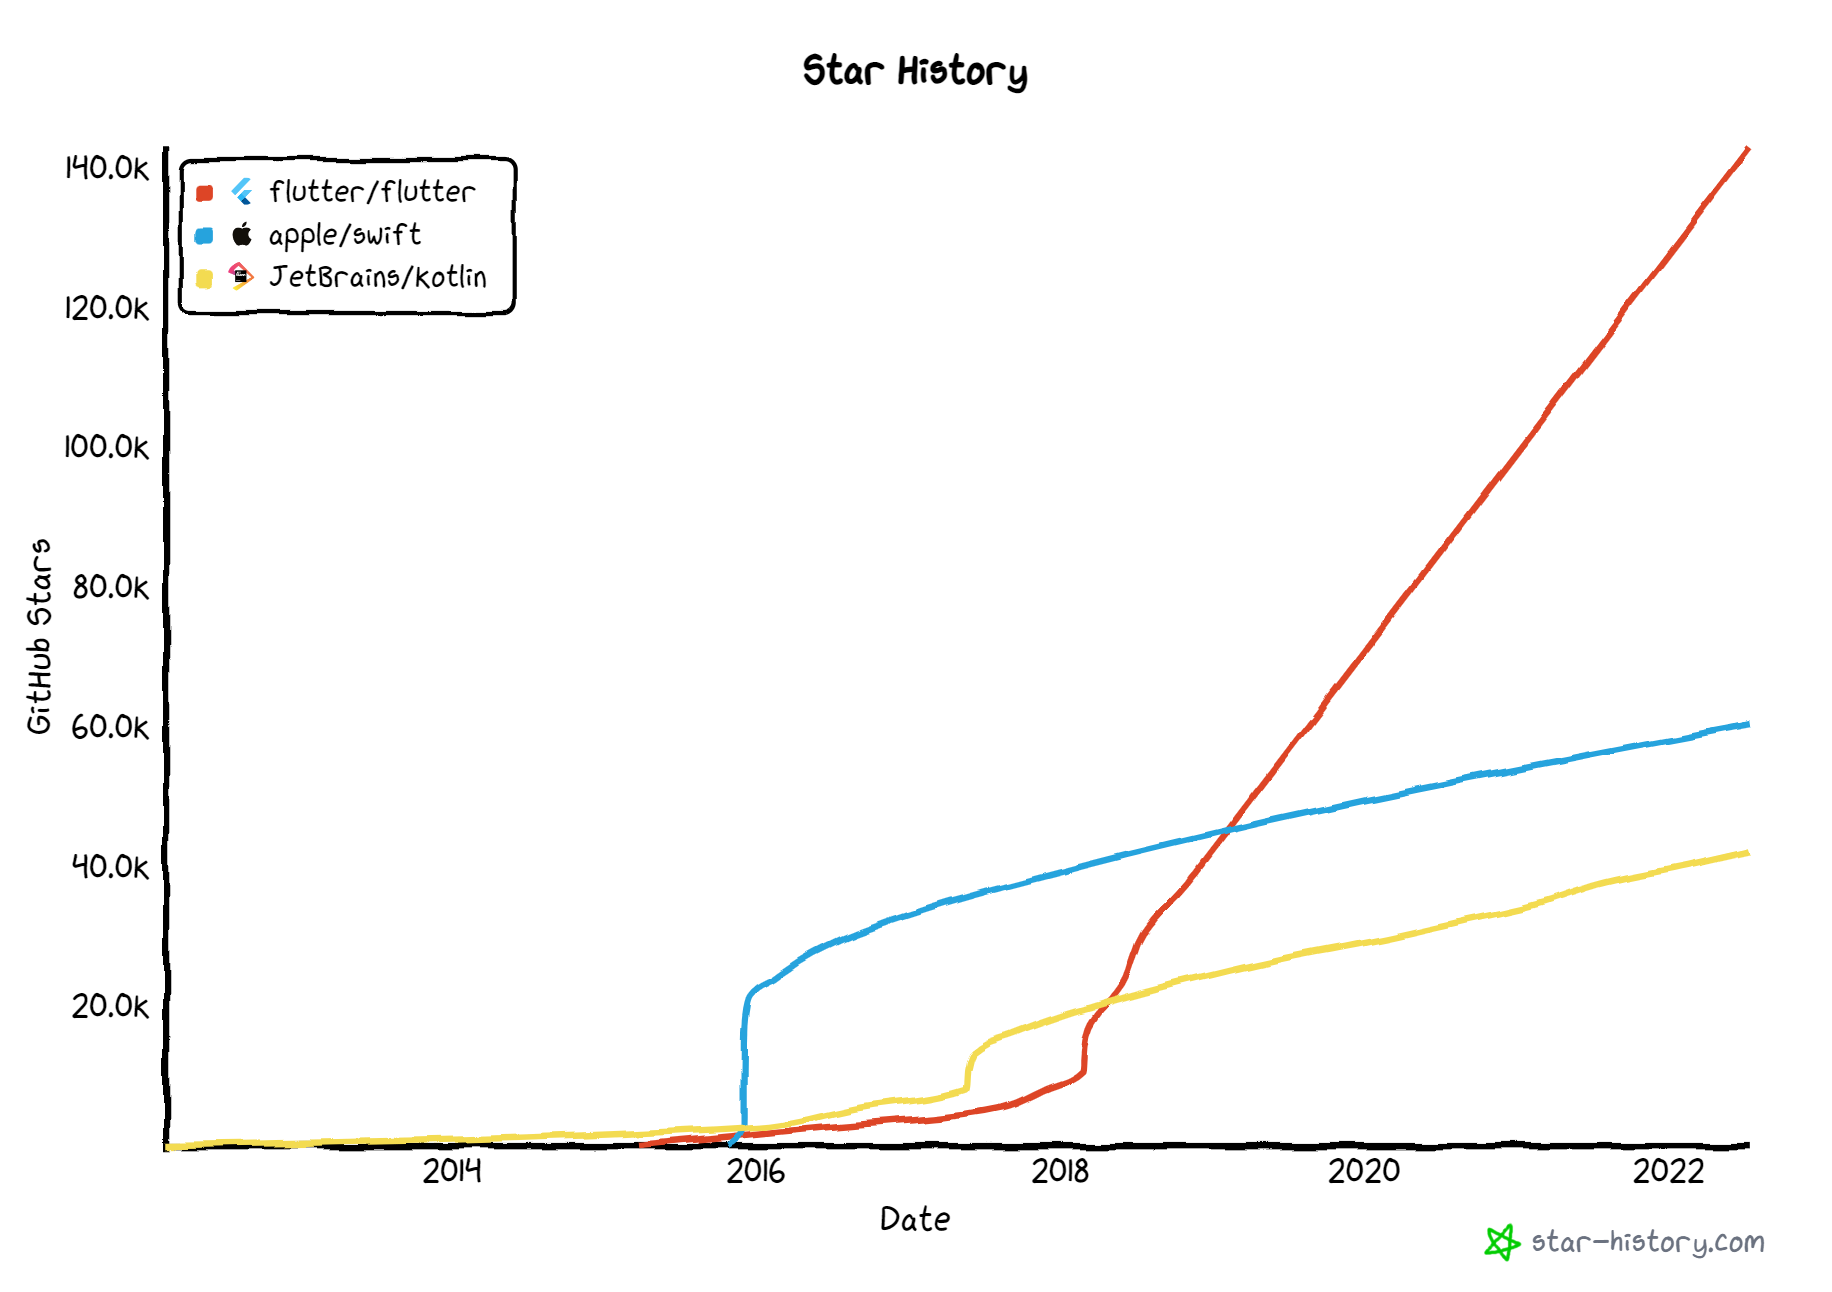
\includegraphics[height=8.5cm,keepaspectratio]{images/star-history_programming languages.png} 
  \caption[Zeitlicher Verlauf von Stars der Github-Repositorys von Swift, Kotlin und Flutter]{Zeitlicher Verlauf von Stars der Github-Repositorys von Swift, Kotlin und Flutter\protect\footnotemark }
  \label{fig:star_history}
\end{figure}
\footnotetext{\url{https://star-history.com/\#flutter/flutter\&JetBrains/kotlin\&apple/swift\&Date}}



Abbildung \ref{fig:star_history} zeigt ein, mit Hilfe der GitHub-Api erstelltes, Diagramm. Darin wird die Anzahl der Stars der Swift, Kotlin und Flutter Repositories im zeitlichen Verlauf angezeigt. 
Besonders gut zu erkennen ist, wie stark das Interesse an Flutter ist. Nach der ersten Ankündigung 2018 und der darauf ersten veröffentlichten Version ist die Zahl der Stars innerhalb von 4 Jahren auf 140 000 angestiegen. Die Repositories für Swift und Kotlin haben im gleichen Zeitraum gerade einmal 20 000 Stars dazu erhalten. Zwar haben Swift und Flutter beide innerhalb des ersten Jahres nach ihrer Vorstellung etwa 30 000 Stars erhalten. Jedoch ist das Interesse an beiden nach einer anfänglichen Phase abgeflacht und verlaufen parallel zueinander.

\subsubsection{Stackoverflow}
Ein anderer Anhaltspunkt für die Größe einer Entwicklergemeinschaft ist die Anzahl der gestellten Fragen auf Stackoverflow. Stackoverflow bietet eine Plattform, um Fragen zu Entwicklungsproblemen zu stellen. Diese können von anderen Entwicklern beantwortet werden. So können generelle Ideen diskutiert und kleine Code-Stücke ausgetauscht werden. Stackoverflow ermöglicht es angemeldeten Nutzern, unter entsprechender Filterung, die Anzahl der gestellten Fragen für einen Suchbegriff zu bestimmen. Hierfür wurde die Anzahl der Fragen bezüglich Kotlin, Swift und Flutter innerhalb der letzten 2 Jahre bestimmt. Zusätzlich wurde auch noch die Anzahl der ingesamt gefundenen Fragen bestimmt. Dabei wurden eventuelle Überschneidungen mit anderen Programmiersprachen, sowie unbeantwortete Fragen heraus gefiltert.

\begin{table}[ht]
\centering
\caption{Anzahl gefundener Fragen pro Programmiersprache}
\begin{tabular}{ |p{3.7cm}||p{5cm}| p{5cm}|}
 \hline
 Programmiersprache & Anzahl gefundener Fragen der letzten 2 Jahre & insgesamt gefundene\\
 \hline
 Kotlin &  105 082 Fragen\tablefootnote{Filter: [kotlin] or [android][kotlin] or [android]-[flutter]-[java] lastactive:2y.. is:question answers:1..} & 920 585 Fragen\\
  \hline
 Swift  & 71 749 Fragen\tablefootnote{Filter: [swift] or [ios][swift] or [ios]-[flutter]-[objectivc] lastactive:2y.. is:question answers:1..} & 670 697 Fragen\\
  \hline
 Flutter & 77 568 Fragen\tablefootnote{Filter:[flutter] or [dart] -[ubuntu] lastactive:2y.. is:question answers:1..} & 115 533 Fragen\\
 \hline
\end{tabular}
\label{tab:evaluations_questions_stackoverflow}
\end{table}

Tabelle \ref{tab:evaluations_questions_stackoverflow} zeigt die ermittelten Werte. Flutter hat hierbei in den letzten zwei Jahren eine ähnlich aktive Community wie Kotlin und Apple. Hier muss jedoch bedacht werden, dass Fragen, die bereits vor dem Untersuchungszeitraum gestellt wurden, innerhalb dieses Zeitraumes nicht erneut gestellt wurden. Deswegen wurde die insgesamt Anzahl der Fragen ebenfalls betrachtet. Hierbei ist die Anzahl sowohl bei Kotlin als auch Swift deutlich höher. Jedoch wurde diese beiden Technologien früher als Flutter veröffentlicht.
Für Flutter zeigt sich, dass in den letzten 2 Jahren eine ähnlich große Community wie für Kotlin und Swift existiert.

\subsubsection{Dokumentation}
Ein weiterer Faktor ist die Dokumentation. Sowohl Flutter als auch Kotlin und Swift veröffentlichen eine umfangreiche und von den Entwicklern dauerhaft aktualisierte Dokumentationsseite. Jedoch besitzt Flutter im Gegensatz zu Android und iOS einen offiziellen zentralen Ort\footnote{\url{https://pub.dev/}}, um nach externen Packages zu suchen. Hier sind neben den offiziellen von Flutter veröffentlichten Repositories, auch von der Community entwickelte Packages verlinkt. In der Summe können hier bereits über 27000 Erweiterungen gefunden werden\footnote{\url{https://pub.dev/packages?q=}}. Neben einem Punktesystem, dass diese bezüglich der Einhaltung von Richtlinien bewertet, werden außerdem die unterstützten Plattformen angezeigt. Zwar gibt es auch Bemühungen ein solches Verzeichnis für Kotlin und Swift einzuführen, jedoch sind diese nicht offiziell von den Entwicklerfirma betrieben und oft nicht vollständig.

Neben der Dokumentation für die Programmiersprache, existieren weitere Dokumentationen für die verschiedenen Entwicklungsansätze. Dabei sind sowohl für den cross-kompilierte, als auch für den native Ansatz eine umfangreiche Dokumentation verfügbar, da sie der Standardentwicklungsmethode der Programmiersprache folgen. Für den gewählten hybriden Ansatz konnte anhand von Anleitungen und Dokumentation der Programmiersprache eine ausreichende Basis gefunden werden. Lediglich der gemischte Ansatz verfügte über keine Dokumentation. Zwar existiert gute Dokumentation für die gewählten Grundlagen und die Web Implementierung, jedoch ist nur wenig Dokumentation für den genauen Ansatz und die Kombination der Technologien vorhanden. Dies wird jedoch durch die Art der Implementierung bedingt, da viele verschiedene gemischte Implementierungen möglich sind. Diese besitzen dabei oft eher einen experimentellen Charakter.

Zusammenfassend wird ersichtlich, dass bei einer normalen Nutzung der Programmiersprache beziehungsweise des Frameworks, eine umfangreiche Dokumentation gefunden werden kann. Je mehr sich jedoch von der normalen Nutzung entfernt wird, desto geringer wird die Dichte an verfügbaren Materialien. 

\subsubsection{Entwickler}
Ein letzter Faktor der zu dieser Kategorie analysiert werden soll, ist die Anzahl der verfügbaren Entwickler. Eine Befragung \cite{statist_used_programming_languages} von 71 547 Entwicklern der Firma Stackoverflow zeigt, dass etwa 9\% Kotlin, 7\% Dart und 5\% Swift beherrschen.
Bei den Programmiersprachen der Webtechnologien, gaben  65\% an, JavaScript zu kennen und 55\% können mit HTML beziehungsweise CSS entwickeln. Diese Zahlen lassen den Schluss zu, dass die Ansätze mit einem hohen Anteil an Web Technologie einen Vorteil haben, da es mehr Entwickler für diese Ansätze gibt. Jedoch wird auch bei diesen Ansätzen mindestens ein Entwickler benötigt, der sich mit den einzelnen Plattformen genauer auskennt. 
Ansonsten ist die Entwicklung eigener plattformspezifischer Funktionalität nicht möglich.

\section{Entwicklungsdauer}
Ein weiteres wichtiges Kriterium bei der Wahl des Ansatzes ist die Entwicklungsdauer, da diese sich auf die Kosten der entwickelten Multi-Plattform-Anwendung auswirkt. Außerdem sollen Applikationen möglichst schnell entwickelt und an den Nutzer verteilt werden können. Daher soll zusätzlich die Zeit betrachtet werden, bis die Applikation beziehungsweise ein Update bei den Nutzern verfügbar ist.

\subsubsection{Programmieraufwand}
Die genaue Entwicklungsdauer ist stark von der Erfahrung der Entwickler und eventuell auftretenden Problemen während der Implementierung abhängig. Folglich ist ein Zeitvergleich hier nicht sinnvoll. Stattdessen soll die Anzahl der geschriebenen Programmzeilen / Lines of Code (LOC) betrachtet werden.
Dafür wurden die einzelnen Daten mit Hilfe des Statistics\footnote{\url{https://plugins.jetbrains.com/plugin/4509-statistic}} Plug-In von JetBrains gesammelt.
Bei den beiden Implementierungen mit Web-Anteil wurde außerdem der notwendig Teil der Web-Implementierung mit angegeben. 
Die gesammelten Daten wurden in drei Teile aufgeteilt: Konfiguration, Benutzeroberfläche und Logik. 
Bei den Implementierungen, welche Flutter benutzen, ist der UI- und Logikcode zusammengefasst, da dies bei Flutter nicht unterschieden werden kann.
Als weiterer Parameter wurde der benötigte Code untersucht, um eine Liste an Objekten anzuzeigen.
Dabei wurde automatisch generierter Code nicht gezählt, sondern nur der tatsächlich geschriebene.

\begin{table}[ht]
\centering
\caption[Programmlänge der verschiedenen Implementierungen in LOC]{Programmlänge der verschiedenen Implementierungen in LOC}
\begin{tabular}{ |p{3.5cm}||p{2.5cm}|p{3.5cm}|p{2.5cm}|p{2.5cm}| }
 \hline
 Programmteile in Lines of Code & gemischte Applikation & cross-kompilierte Applikation & native\break Applikation & hybride\break Applikation \\
 \hline
 Gesamte\break Anwendung       &   2391(App) + 1533(Web) &   2100 & 3138 & 215(App) + 2814(Web)\\
  \hline
 Konfigurationscode  & 42 + 268& 32& 229& 30 + 357\\
  \hline
 Oberflächencode &\multirow{2}{*}{2349 + 1265}  &\multirow{2}{*}{2068}  & 1958& 86 + 1768\\
  \cline{1-1}
  \cline{4 -5}
 Funktionalität \& Logik & & & 951& 99 + 689\\
  \hline
 Beispiel: Liste an Gegenständen & 65(App) & 65 & 178 & 71(Web)\\
  \hline
\end{tabular}
\label{tab:lines_of_code}
\end{table}

Die in Tabelle \ref{tab:lines_of_code} zu sehende Aufschlüsselung zeigt, dass Flutter insgesamt die wenigsten Zeilen Code benötigt. 
Dabei werden gerade einmal 32 Zeilen Code Konfiguration benötigt. 
Der Rest sind knapp 2000 Zeilen Code mit Benutzeroberfläche und Logik.
Den höchsten Programmieraufwand in diesem Vergleich benötigt der gemischte Ansatz. Er kommt insgesamt auf circa 4000 Zeilen Code und benötigt damit rund doppelt so viel wie die Flutter Implementierung. 
Die native und die hybride Implementierung haben in etwa gleich viele Zeilen Code und liegen mit rund 3000 Zeilen Code zwischen den zwei anderen Implementierungen.

Bei dem zusätzlich betrachteten Beispiel, einer dynamischen Liste für Gegenstände ohne feste Länge, ist die Flutter Implementierung ebenfalls die Kürzeste. Dabei werden gerade einmal 65 Zeilen Code benötigt, wovon 55 Zeilen auf die Anzeige eines Gegenstandes und gerade einmal 10 Zeilen Code auf die Liste entfallen. Ähnlich verhält sich dies bei der Implementierung mit einer Webseite. Einzig die native Kotlin Applikation hat hierbei einen erhöhten Aufwand. Dabei fallen 75 Zeilen für das Design und weitere 83 Zeilen für die Steuerung der Liste an. Ein Großteil davon ist der Adapter, der benötigt wird, um die Liste zu steuern. 

Ebenfalls muss beachtet werden, wie viele Implementierungen je Ansatz benötigt werden. So ist bei dem gemischten und dem cross-kompilierten Ansatz lediglich die eine vorgestellte Implementierung nötig. Bei dem nativen Ansatz muss jedoch pro unterstützter Plattform eine eigenständige Implementierung erstellt werden. Bei der hybriden Applikation, wie sie in dieser Arbeit umgesetzt wurde, ist zwar die umgebende Applikation ebenfalls für jede Plattform zu implementieren, jedoch hat die Implementierung einen deutlich geringeren Umfang, da der Teil der Web-Anwendung lediglich einmalig zu programmieren ist.  

Es wurde gezeigt, dass eine cross-kompilierte Lösung mit Flutter deutlich weniger Zeilen Code als die anderen Implementierungen benötigt.
Sollte jedoch bereits eine Web-Anwendung existieren, reduziert sich der Implementierungsaufwand der hybriden Aufwand auf knapp 200 Zeilen Code und die gemischte Implementierung halbiert sich in etwa. Dadurch können diese beiden Implementierungen dann ebenfalls eine gute Alternative zu den anderen Ansätzen darstellen. Muss diese jedoch erst erstellt werden, ist gerade der gemischte Ansatz mit einem erhöhten Aufwand verbunden. Außerdem wurde festgestellt, dass mit mehr unterstützten Plattformen der native Ansatz sich im Aufwand multipliziert.

\subsubsection{Zeit bis zur Veröffentlichung der App und von Updates }
Die Entwicklungsdauer wirkt sich auch auf die Dauer bis zur Veröffentlichung einer ersten Version aus.
Je früher eine Anwendung veröffentlicht werden kann, desto früher können Kunden die Applikation nutzen und bei einer kommerziellen Nutzung folglich auch Umsatz produzieren.

Hier haben die gemischte und die hybride Implementierung den Vorteil, dass bei einer bereits bestehenden Webseite, die Zeit bis zur Veröffentlichung einer ersten Version sehr gering ist, da bereits wenige Zeilen Code die Webseite in der App anzeigen. Zu einem späteren Zeitpunkt können mehr Funktionalitäten und Optimierungen in kommende Versionen hinzugefügt werden. Wenn jedoch keine Webseite besteht, ist die anfängliche Dauer vergleichbar, beziehungsweise etwas höher als bei der cross-kompilierten Implementierung. Lediglich die native Implementierung benötigt durch das Erstellen der verschiedenen Plattform-Applikation deutlich mehr Zeit. Dies kann zwar durch zusätzliche Entwickler begrenzt werden, jedoch steigen dadurch die Entwicklungskosten.

Bei der Veröffentlichung von Updates zeigt sich ein weiterer Vorteil der Nutzung einer Webseite innerhalb einer Applikation. So können Updates auf der Webseite sofort verteilt werden und müssen nicht über den App-Store der verschiedenen Geräte verteilt werden. Die Veröffentlichung von Apps oder deren Updates kann dabei zwischen einem Tag und einer Woche dauern\footnote{\url{https://developer.apple.com/app-store/review/}} \footnote{\url{https://qr.ae/pvu0ud}}. Diese Zeit wird dafür bei jeder Änderung an der App bei allen vier Ansätzen benötigt.

\section{Benutzeroberfläche}
Die Bewertung einer Benutzeroberfläche ist stark von den persönlichen Präferenz abhängig. So empfinden Nutzer unterschiedlich, was eine gute Benutzeroberfläche ausmacht. Folglich soll in dieser Arbeit nicht auf das genaue Aussehen eingegangen werden, sondern auf einige allgemeine Eigenschaften der unterschiedlichen Benutzeroberflächen.

\subsubsection{Aussehen der Applikationen}
Grundsätzlich ist das Aussehen der Applikation vor allem davon abhängig, wie viel Zeit investiert wird, um ein angestrebtes Design zu erhalten. Um die unterschiedlichen Startseiten vergleichbar zu halten, wurde deswegen eine Maximalzeit für die Verwirklichung des Design festgelegt. Diese Maximalzeit orientiert sich an der benötigten Entwicklungszeit der entsprechenden Web-Ansicht. Dafür wurde außer für den Schriftzug mit Farbverlauf keine externen Design-Pakete oder Erweiterungen benutzt. Eine zusätzliche Anforderung war dabei, dass die Seiten für unterschiedliche Bildschirmgrößen benutzbar sein müssen.

\begin{figure}[ht]
  \centering
  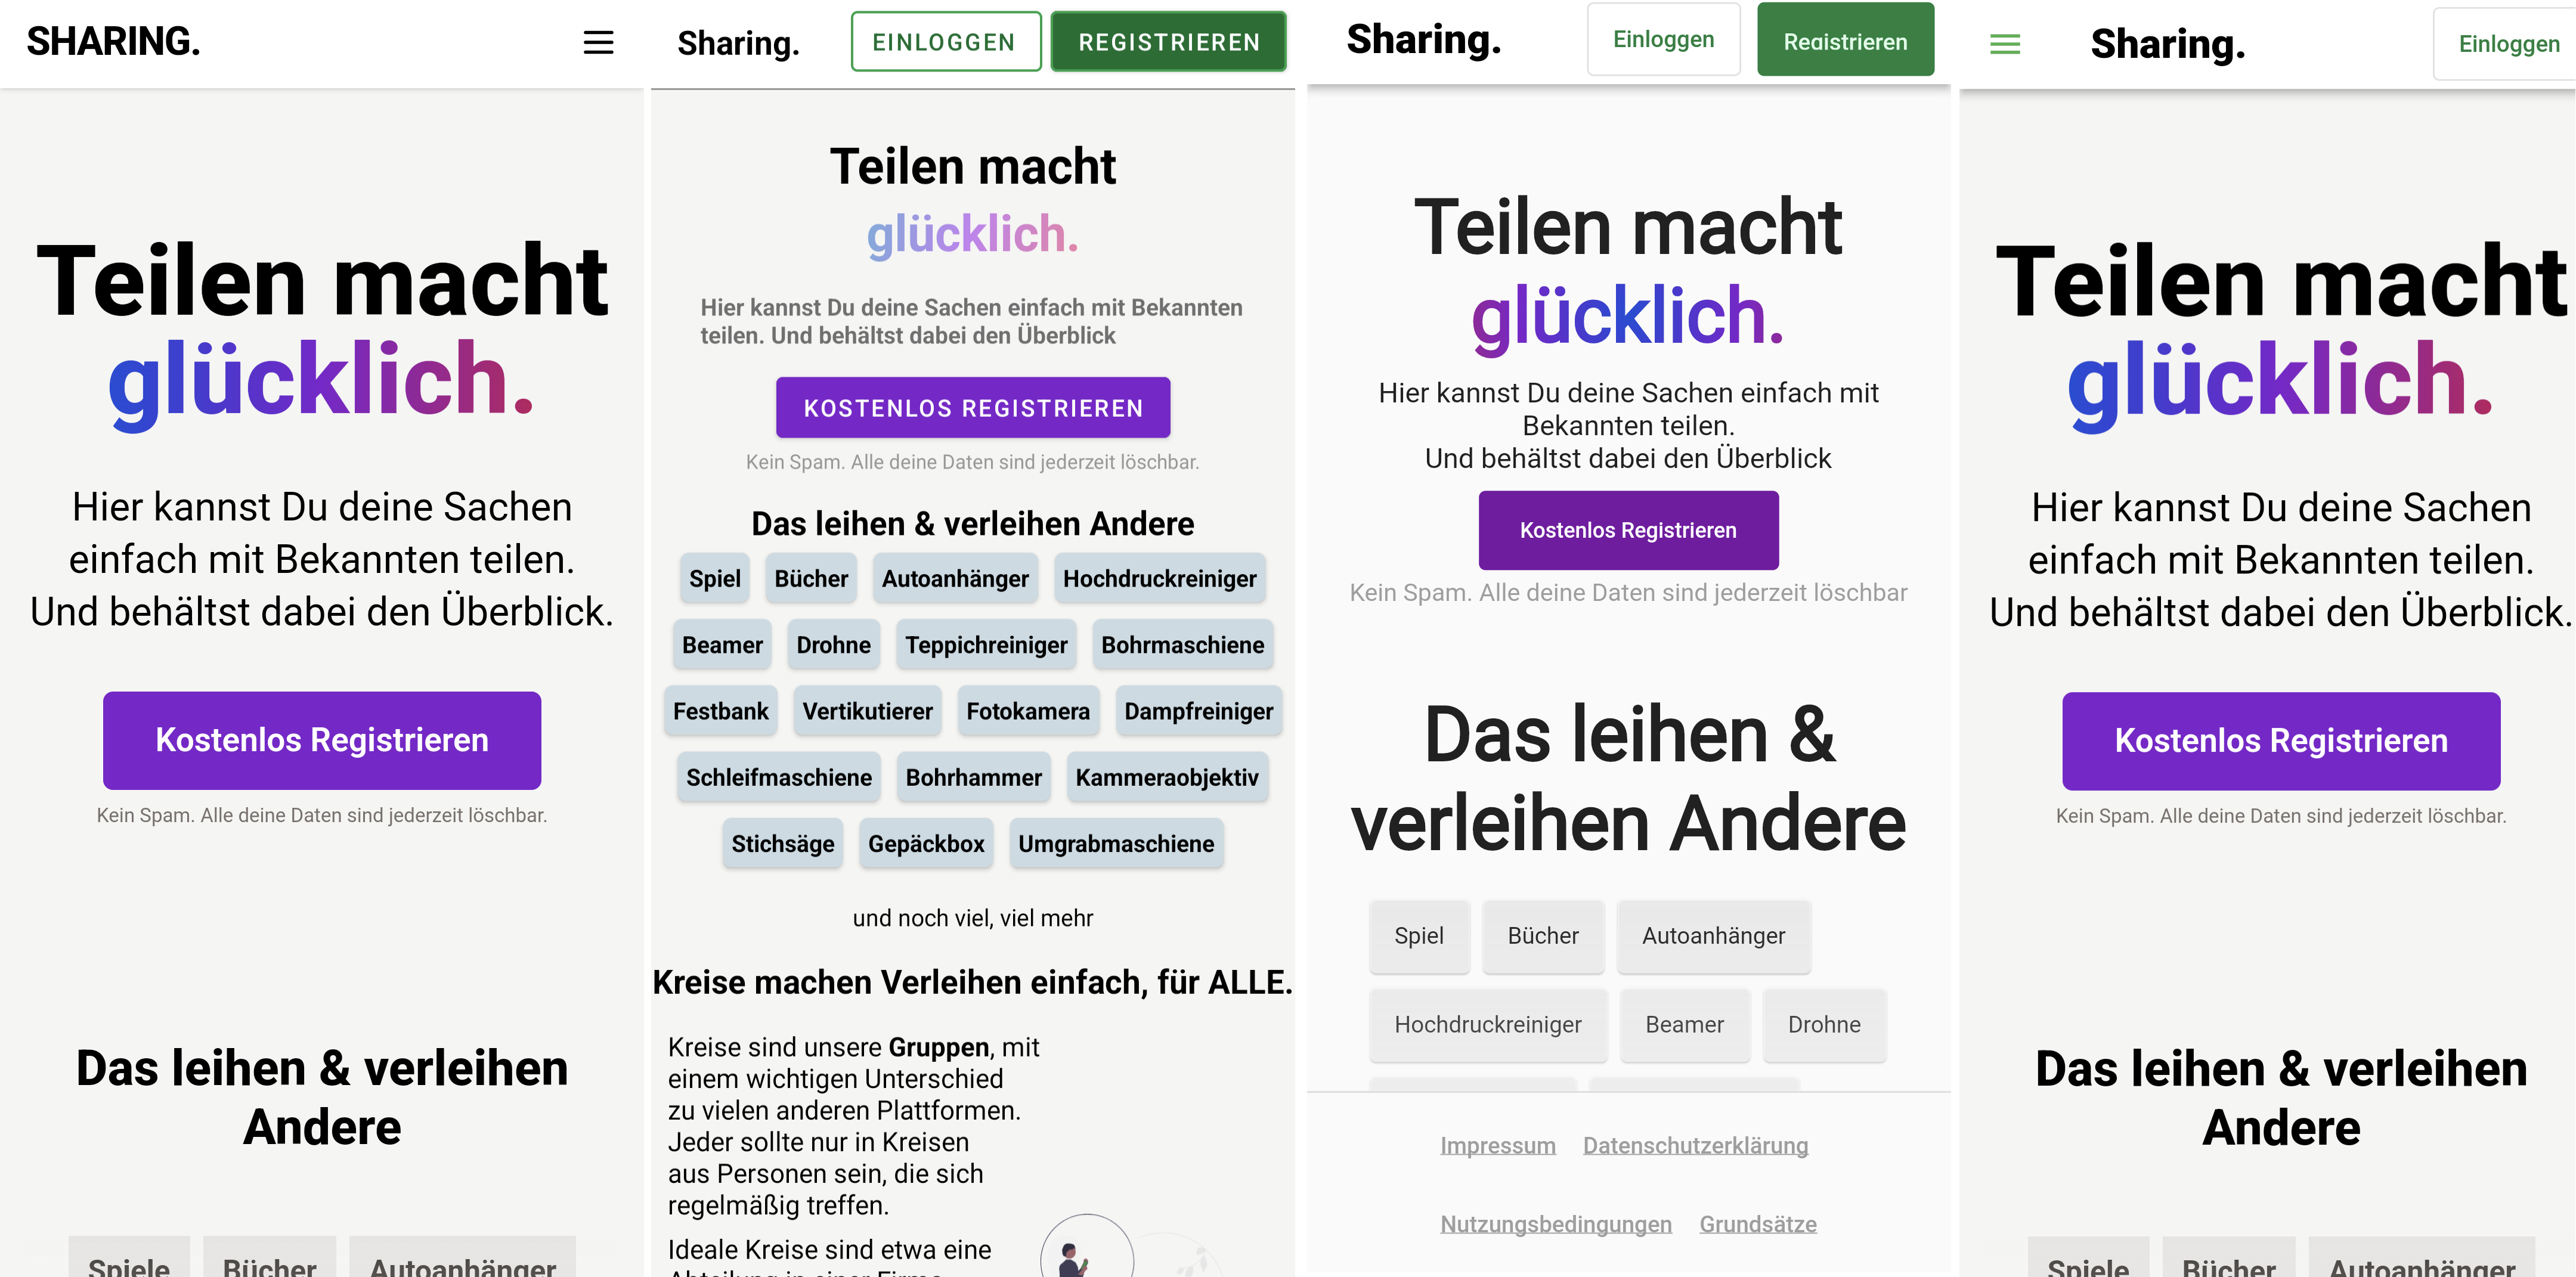
\includegraphics[height=7cm,keepaspectratio]{images/Startbildschirm_vergleich.png} 
  \caption[Vergleich des Startbildschirms der Implementierungen]{Vergleich des Startbildschirms der Implementierungen.\break Von links nach rechts: Hybride-Applikation, native Kotlin Applikation, Flutter Cross-Plattform-Applikation, Flutter Hybride Applikation}
  \label{fig:startscreen}
\end{figure}

In Abbildung \ref{fig:startscreen} sind die Startbildschirme der verschiedenen Anwendungen zu sehen. Dabei zeigen das erste und letzte Bild die Startseite der Webseite. Die zwei mittleren Bilder zeigen die im App-Code definierten Seiten. Grundsätzlich kann dabei festgestellt werden, dass die Seiten ähnlich aussehen, lediglich die Größe des Textes unterscheidet sich zwischen den Versionen stark.

Bei dem ersten Bildschirm, welcher von der hybriden Applikation stammt, musste am Design der Applikation nicht viel angepasst werden, da die Webseite bereits für die Nutzung an ein mobiles Endgerät angepasst war. Jedoch fallen bei der Benutzung Unterschiede zur nativen beziehungsweise Flutter Entwicklung auf. 
Um dies zu verdeutlichen zeigt Abbildung \ref{fig:sidemenu} die Seitenmenüanzeigen der Flutter-Anwendung (links) und der Webimplementierung (rechts). Hierbei ist klar zu erkennen, dass die Web-Implementierung für PC Nutzer ausgelegt ist, da das Menü für eine Anklick-Bedienung optimiert ist. 
Im Gegensatz dazu kann das Seitenmenü bei der Flutter Implementierung über eine Wischgeste geöffnet werden und wird dabei über den gesamten Gerätebildschirm angezeigt, während bei der Webseite das Menü nur innerhalb des Web-Containers angezeigt wird. Dadurch erhält der Nutzer in der Flutter Applikation den Eindruck, dass sich das Menü über die restliche UI legt. 
\begin{figure}[ht]
  \centering
  \includegraphics[height=7cm,keepaspectratio]{images/Seitenmenü_vergleich.png} 
  \caption[Vergleich des Seitenmenüs der nativen und hybriden Applikation]{Vergleich des Seitenmenüs bei nativer Implementierung (links) und JavaScript Implementierung (rechts)}
  \label{fig:sidemenu}
\end{figure}

Während auf der Webseite eine umfangreiche Design-Implementierung genutzt wurde, um das Aussehen der Anwendung zu verändern, wurden bei der nativen Kotlin und den Flutter Implementierungen lediglich die Farben und Textgröße angepasst. Dies wurde gemacht, um einen Eindruck für die Standardkonfiguration des Design der verschiedenen Implementierungen vergleichen zu können. Bei der Flutter Implementierung wirken die Elemente im Gegensatz zur nativen Implementierung moderner und besser an ein Smartphone angepasst. Dies wird deutlich, wenn die Login-Seite verglichen wird.

\begin{figure}[ht]
  \centering
  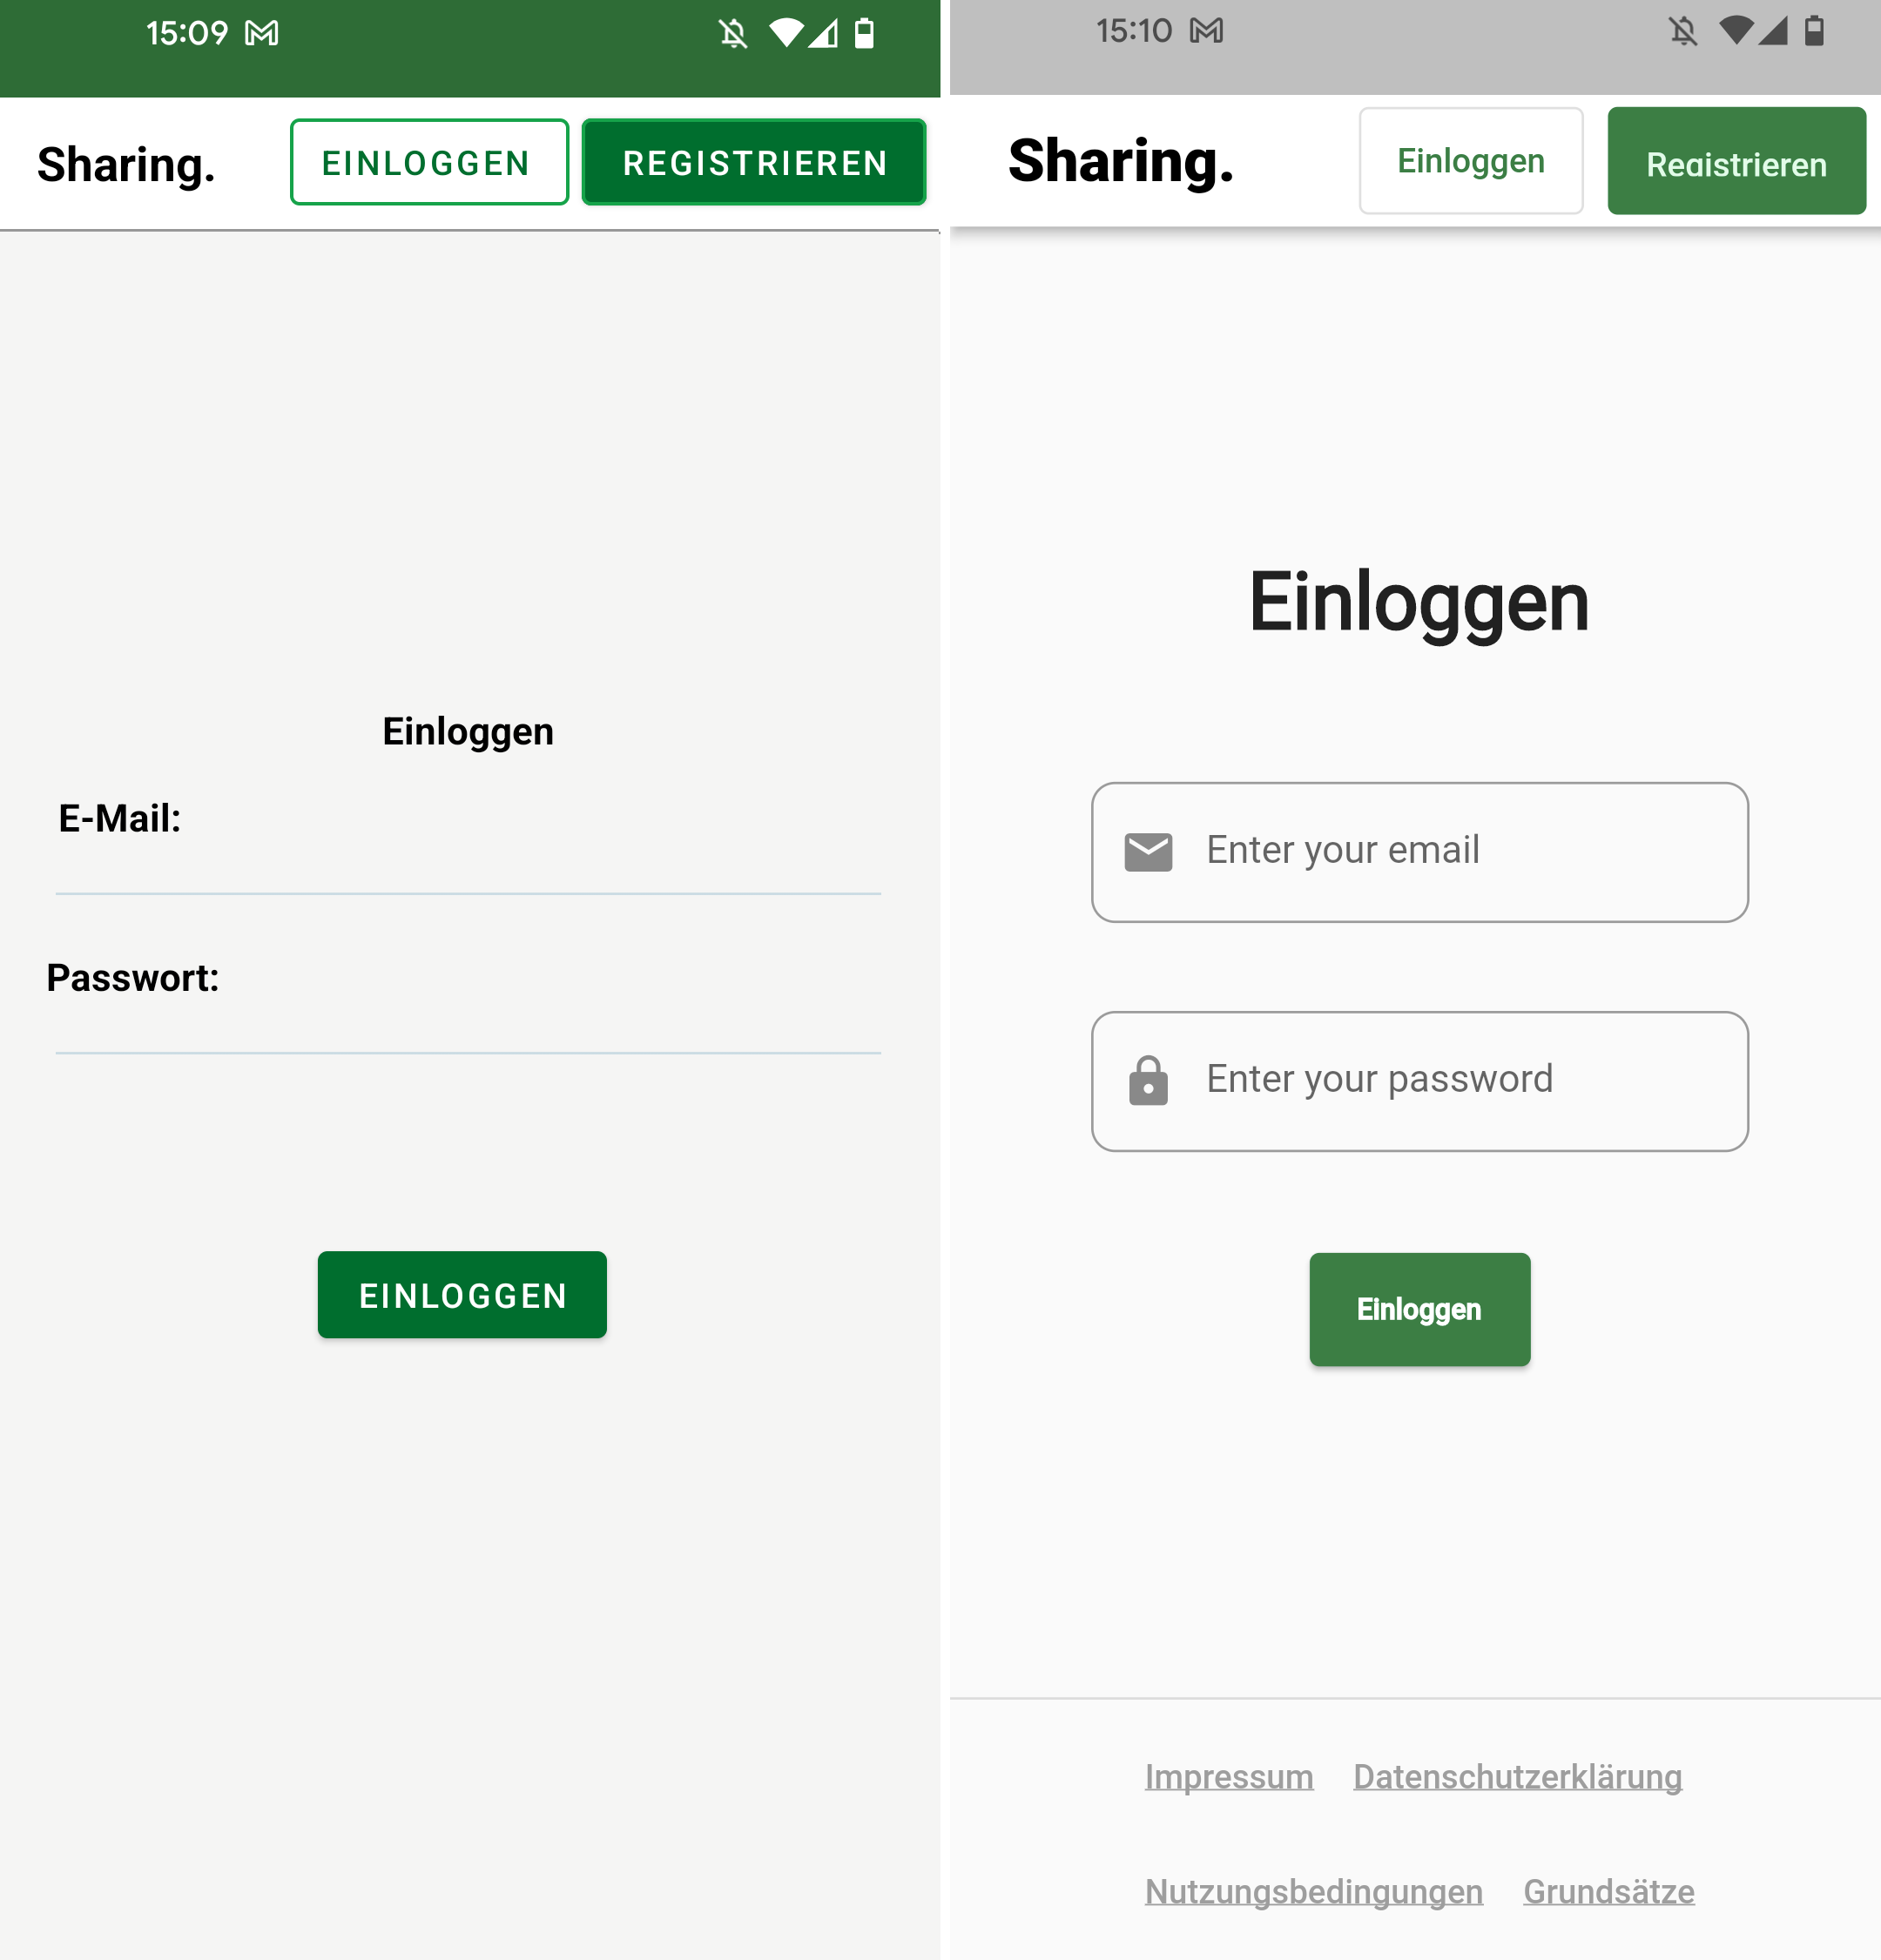
\includegraphics[height=7cm,keepaspectratio]{images/Login_vergleich.png} 
  \caption[Vergleich des Login-Bildschirms von Kotlin und Flutter Implementierung.]{Vergleich des Login-Bildschirms von Kotlin (links) und Flutter (rechts) Implementierung}
  \label{fig:loginscreen}
\end{figure}

In Abbildung \ref{fig:loginscreen} sind die Login-Seiten der nativen und des cross-kompilierten Ansatzes zu sehen. Dabei zeichnet sich Flutter durch ein besseres \"Out-of-the-Box\" Design-Paket aus. So ist das Input Feld bei der Koltin Implementierung  lediglich durch ein Strich definiert und kann dadurch für einen Nutzer schwer zu finden sein. Flutter hingegen hat als Standardinputfeld ein umrahmtes Feld, dass durch hinzufügen von Werten auf vordefinierten Attributen beliebig und einfach im Style angepasst werden kann. Bei der nativen Implementierung ist dies zwar ebenfalls möglich, allerdings entsteht dadurch zusätzlicher Aufwand.

Während der Entwicklung konnte festgestellt werden, dass mit genügend Zeit und den richtigen Erweiterungen, jede Benutzeroberfläche in das gewünschte Format zu bringen ist. Vor allem bei der Unterstützung unterschiedlicher Bildschirmgrößen benötigte jedoch die native Anwendungen umfangreiche Anpassungen, während dies bei den anderen Ansätzen deutlich unkomplizierter zu erreichen war. Flutter unterstütze die Verwirklichung einer gut aussehenden Benutzeroberfläche insofern, dass die Standardkonfiguration Googles Design-Paket Material3\footnote{\url{https://m3.material.io/}} nutzt.

\subsubsection{Konsistenz über Plattformen hinweg}
Ein weiteres Ziel bei der Entwicklung der Benutzeroberfläche ist die Konsistenz über Plattformen hinweg.
Dabei soll der Nutzer keinen Unterschied bemerken, wenn er von einer Plattform zur anderen wechselt. 
Das Risiko solcher Inkonsistenzen ist bei unterschiedlichen Implementierungen für die einzelnen Plattformen höher, als wenn eine einzelne Code-Basis verwendet werden kann.

Dementsprechend haben Implementierungen, die für mehrere Plattformen wieder verwendet werden können einen positiven Einfluss auf die Konsistenz.
Auf die in dieser Arbeit vorgestellten Implementierungen bezogen, bedeutet dies, dass die reine native Implementierung eine höhere Gefahr von Inkonsistenz besitzt, als die Hybride, Gemischte oder Cross-kompilierte.
Dabei ist zu erwähnen, dass auch die nativen Applikationen einen hohen Grad an Konsistenz erreichen können. Dies erfordert jedoch wieder einen höheren Aufwand und eine enge Zusammenarbeit der Entwickler während der Implementierung der verschiedenen Plattformen.

\section{Funktionalität}
Als letztes Kriterium wird die Funktionalität der einzelnen Ansätze betrachtet. Dabei soll neben der Plattformabdeckung, die Möglichkeiten zur Nutzung von offline Funktionalität und Plattformfunktionalität betrachtet werden.

\subsubsection{Plattformabdeckung}
Wie bereits erwähnt, sind nativ entwickelte Applikationen immer nur für eine Plattform verwenbar. Sie haben dementsprechend auch wenig wiederverwendbaren Code. Allerdings kann für jede Plattform eine native Applikation geschrieben werden und folglich können alle Plattformen abgedeckt werden.

Bei der hybriden Implementierung muss ebenfalls eine Applikation für jede Plattform geschrieben werden, jedoch kann der Web-Code auf den unterschiedlichen Plattformen wiederverwendet werden. Grundsätzlich können auch bei diesem Ansatz alle Plattformen unterstützt werden, dabei müssen jedoch die Anforderungen der verschiedenen App-Stores beachtet werden. Denn wie bereits erwähnt, verlangt beispielsweise Apple, dass Apps den Großteil der Funktionalität intern abbilden. Eine Implementierung, wie sie hier vorgestellt wurde, würde wahrscheinlich abgelehnt werden.

Flutter bietet eine Unterstützung für alle aktuell verfügbaren mobilen Plattformen an. Außerdem arbeiten sie an einer Möglichkeit, Flutter auch auf Embedded-Geräten auszuführen\footnote{\url{https://flutter.dev/multi-platform/embedded}}.
Somit können alle Plattformen abgedeckt werden. Jedoch kann die Plattformunterstützung der eigenen Applikation durch genutzte Bibliotheken eingeschränkt werden. Beispielsweise war die, in dieser Arbeit vorgestellte, cross-kompilierte Implementierung lediglich mit fünf der sechs Plattformen kompatibel, da der genutzte GraphQL-Client keine Web-Version unterstützt.

Die gemischten Implementierung unterstütze noch weniger Plattformen. So konnte aufgrund des genutzten Web-Containers die Applikation lediglich auf Android und iOS genutzt werden.
Daher ist es eventuell sinnvoll, vor der Wahl eines Ansatzes auch benötigte Technologien zu recherchieren und die verfügbaren Bibliotheken zu analysieren, um derartige Probleme bereits vor dem Start der Implementierung zu identifizieren.


\subsubsection{Offline Funktionalität}
Es gibt einige Fälle in denen der Nutzer eine Applikation benutzen will, auch wenn er aktuell über keine aktive Internetverbindung verfügt. In diesem Fall benötigt die Applikation eine offline Funktionalität.

Wie in dieser Arbeit erwähnt, sind die Implementierungen die eine Webseite als Teil ihrer Implementierung haben offline stark eingeschränkt oder haben keine Funktionalität. Im Falle der gemischten Implementierung kann eine offline Funktionalität zumindest teilweise erreicht werden, indem bei einer fehlenden Internetverbindung durch Flutter implementierte Seiten angezeigt werden. Die native und cross-kompilierte Lösung haben hier den Vorteil, dass ihre Benutzeroberfläche unabhängig von einer aktiven Internetverbindung nutzbar ist. Zwar kommen die angezeigten Daten von einem Server, jedoch können diese lokal zwischengespeichert werden. Diese Lösung ist dabei sowohl für die native, kross-compilierte und gemischte Implementierung möglich. 

Zu beachten ist, dass einige hybride Frameworks Daten und Benutzeroberfläche lokal auf dem Gerät speichern und dadurch eine offline Funktionalität möglich wäre. Allerdings verschwinden dadurch die Vorteile der Nutzung einer online Version, wie etwa die einfache Verteilung von Updates.

\subsubsection{Nutzung von Plattformfunktionalität}
Wie bei der Vorstellung der unterschiedlichen Implementierungen aufgezeigt wurde, kann mit der richtigen Implementierung die Nutzung der Plattformfunktionalität bei jeder der vier Implementierungen ermöglicht werden. Jedoch konnte aufgezeigt werden, dass die Nutzung mit unterschiedlichen Aufwand verbunden ist. So ist dies bei der nativen Implementierung am einfachsten umsetzbar. Auch der cross-kompilierte und der gemischte Ansatz können vollständig, wie in Kapitel 4.3.3 vorgestellt, auf die nativen Funktionen zugreifen. Ebenfalls kann der hybride Ansatz native Funktionalität nutzen, muss dafür jedoch eine Javascript-Schnittstelle nutzen. Dies birgt Gefahren, die beachtet und abgeschätzt werden müssen (siehe Kapitel 4.2.2). Hier hat der gemischte Ansatz insofern den Vorteil gegenüber dem hybriden, dass die Web-Ansichten, die Plattformfunktionalität benötigen, durch Flutter-Seiten ersetzt werden können. Somit ist ein sicherer und einfacher Zugriff wie bei der cross-kompilierten Implementierung möglich.

\chapter{Fazit}
\section{Flutter vs. Native Android}
\section{Nativ vs. Hybrid vs. Cross-Plattform}

\section{Entscheidung zu unterschiedlichen Ansätzen}

------
Schon genauere Erklärung:
Wenn man die Idee zu einer App hat, gibt es die große Frage, wie man nun anfängt und welche Programmiersprache / Framework man wählt. Hierfür gibt es ganz verschiedene Ansätze.  

Jedoch noch grundlegender ist die Frage nach der Plattform. Es gab lange Zeiten in der Applikationsentwicklung, dass nur eine Webversion veröffentlicht wurde. Mittlerweile nutzen jedoch viele Menschen nur noch ihr Smartphone und wollen dementsprechend auch nur mit mobilen Versionen auskommen. Man kann natürlich auch im Web veröffentlichte Applikationen auf dem Handy nutzen, jedoch gibt es hier zwei Sachen, die dazu führen können, dass man eine eigenständige App entwickelt.
1. Eine auf mobile angepasste UI. - Auch wenn es heutzutage in fast jedem Framework und vor allem in den gängigen UI-Frameworks verschiedene Ansätze gibt, die eine recht nutzerfreundliche Version für Mobilgeräte anbieten, oder manchmal auch sogar komplett eigenständige Oberflächen für mobil angezeigt werden, so kann es doch sinnvoll sein, nochmal extra angepasste UI in Form einer Applikation nativ für die Geräte zu entwickeln. Dadurch kann man gezielt Oberflächen für die Plattformen bauen und dabei auf Plattform eigene Design Unterstützungen zugreifen. Die eine Bedienung um einiges besser machen.
2. Nutzung von Hardwarefunktionalität. -  Ein noch viel wichtigerer Punkt ist es, Funktionalität die mobile Endgeräte anbieten, zu nutzen, die etwa auf einem PC nicht nutzbar sind. Dazu zählen unter anderem GPS-Nutzung, Kamerafunktionalitäten, Bluetooth-Verbindungen,.... Diese können zwar manchmal auch durch einen PC geboten sein, jedoch ist es hier nicht gegeben, während man bei einem Smartphone sicher davon ausgehen kann, dass die Kamera genutzt werden kann. So können einige Geschäftsprozesse der Applikationen vereinfacht oder umgestaltet werden, so dass eine Nutzung der Applikation für den Nutzer einfacher wird, bzw. es können auch neue Funktionalitäten daraus ergeben, die es eventuell davor nicht gab.

Wenn nun die Entscheidung getroffen wurde, dass man eine mobile Applikation entwickeln will, so gibt es nun verschiedene Ansätze bzw. Frameworks, die zur Verfügung stehen. Dabei gibt es viele verschiedene Frameworks die auf den ersten Blick das selbe tun, aber doch recht unterschiedlich sein können und unter gewissen Ummständen sich manche besser eignen als andere. 
Eine der ersten Fragen die dabei im Raum steht. Gibt es bereits eine Webversion der Applikation.
Wenn nicht, so kann es von Anfang an spannend sein, ein Framework zu wählen, dass wie Flutter eine Cross-Plattform-Applikation erzeugt, wo auch eine Webversion mit gehostet werden kann.
Falls es bereits eine Webversion geben, so geht der Weg eher in Richtung von Nativen- bzw. Hybriden Applikationen, da meißt nur noch einzelne Teile der Applikation entwickelt werden müssen. Dies ist jedoch auch kein Grund eine Cross-Plattform-Entwicklung auszuschließen, da dadurch nur ein Code geschrieben werden muss um etwa beide vorherschenden mobilen Plattformen abzudecken: iOS und Android.

'''Hier könnte man so ein Art Diagramm machen mit Fragen und dann Entscheidungswegen. So nach dem Motto finde dein Framework zur entwicklung einer mobilen Applikation.'''



\vfill
\pagebreak

\appendix

% ----------------------------------------------------------------------------------------------------------
% Abkürzungsverzeichnis (optional, bitte nur wenn sinnvoll)
% ----------------------------------------------------------------------------------------------------------
%\listoftables
\addchap{Abkürzungsverzeichnis}
\begin{acronym}[KDE]
\acro{BA}[BA]{Bachelorarbeit}
\end{acronym}
\vfill
\pagebreak


% ----------------------------------------------------------------------------------------------------------
% Filter fuer Literatur und Quellen definieren
% ----------------------------------------------------------------------------------------------------------

\defbibheading{Literatur}{\addchap{Literaturverzeichnis}} 
\defbibheading{Quellen}{\addchap{Internetquellenverzeichnis}} 
  
\defbibfilter{Literatur}{\not\keyword{online}} 
\defbibfilter{Quellen}{\keyword{online}} 


% ----------------------------------------------------------------------------------------------------------
% Literatur
% ----------------------------------------------------------------------------------------------------------

\printbibliography[heading=Literatur,filter=Literatur] 
\vfill

\pagebreak


% ---------------------------------------------------------------------------------------------------------- 
% Internetquellen 
% ---------------------------------------------------------------------------------------------------------- 

\printbibliography[title = {Quellenverzeichnis}, heading=Quellen,filter=Quellen] 

\pagebreak 

% ----------------------------------------------------------------------------------------------------------
% Anhang
% ----------------------------------------------------------------------------------------------------------
\appendix


\chapter{Anhang}

% \input{inhalt/suppl}


\pagebreak


% % ----------------------------------------------------------------------------------------------------------
% % Eigenschtändigkeitserklaerung
% % ----------------------------------------------------------------------------------------------------------
\thispagestyle{empty}
\chapter*{Erklärung zur Bachelorarbeit}

\bigskip
\bigskip 
\bigskip 

\textbf{1.}\\[1ex]
    Mir ist bekannt, dass dieses Exemplar der Abschlussarbeit als Prüfungsleistung in das Eigentum der Ostbayerischen Technischen Hochschule Regensburg übergeht.

\textbf{2.}\\[1ex]
    Ich erkläre hiermit, dass ich diese Abschlussarbeit selbständig verfasst, noch nicht anderweitig für Prüfungszwecke vorgelegt, keine anderen als die angegebenen Quellen und Hilfsmittel benutzt sowie wörtliche und sinngemäße Zitate als solche gekennzeichnet habe.

\bigskip 
\bigskip 
\bigskip 
~\hfill\begin{minipage}{.5\textwidth}

Regensburg, den \today

\bigskip 
\bigskip

\line(1,0){200}
\newline
\stud

\end{minipage}




\end{document}